% !TEX TS-program = pdflatex
\documentclass[notoc,notitlepage]{tufte-book}
% \nonstopmode % uncomment to enable nonstopmode

\usepackage{classnotetitle}

\title{PMATH450 --- Lebesgue Integration and Fourier Analysis}
\author{Johnson Ng}
\subtitle{Classnotes for Spring 2019}
\credentials{BMath (Hons), Pure Mathematics major, Actuarial Science Minor}
\institution{University of Waterloo}

\setcounter{secnumdepth}{3}
\setcounter{tocdepth}{3}

\renewcommand{\baselinestretch}{1.1}
\usepackage{geometry}
\geometry{letterpaper}
\usepackage[parfill]{parskip}
\usepackage{graphicx}

% Essential Packages
\usepackage{makeidx}
\makeindex
\usepackage{enumitem}
\usepackage[T1]{fontenc}
\usepackage{natbib}
\bibliographystyle{apalike}
\usepackage{ragged2e}
\usepackage{etoolbox}
\usepackage{amssymb}
\usepackage{fontawesome}
\usepackage{amsmath}
\usepackage{mathrsfs}
\usepackage{mathtools}
\usepackage{xparse}
\usepackage{tkz-euclide}
\usetkzobj{all}
\usepackage[utf8]{inputenc}
\usepackage{csquotes}
\usepackage[english]{babel}
\usepackage{marvosym}
\usepackage{pgf,tikz}
\usepackage{pgfplots}
\usepackage{fancyhdr}
\usepackage{array}
\usepackage{faktor}
\usepackage{float}
\usepackage{xcolor}
\usepackage{centernot}
\usepackage{silence}
  \WarningFilter*{latex}{Marginpar on page \thepage\space moved}
\usepackage{tcolorbox}
\tcbuselibrary{skins,breakable}
\usepackage{longtable}
\usepackage[amsmath,hyperref]{ntheorem}
\usepackage{hyperref}
\usepackage[noabbrev,capitalize,nameinlink]{cleveref}

% xcolor (scheme: base16 eighties)
\definecolor{base16-eighties-dark}{HTML}{2D2D2D}
\definecolor{base16-eighties-light}{HTML}{D3D0C8}
\definecolor{base16-eighties-magenta}{HTML}{CD98CD}
\definecolor{base16-eighties-red}{HTML}{F47678}
\definecolor{base16-eighties-yellow}{HTML}{E2B552}
\definecolor{base16-eighties-green}{HTML}{98CD97}
\definecolor{base16-eighties-lightblue}{HTML}{61CCCD}
\definecolor{base16-eighties-blue}{HTML}{6498CE}
\definecolor{base16-eighties-brown}{HTML}{D47B4E}
\definecolor{base16-eighties-gray}{HTML}{747369}

% hyperref Package Settings
\hypersetup{
    bookmarks=true,         % show bookmarks bar?
    unicode=true,          % non-Latin characters in Acrobat’s bookmarks
    pdftoolbar=false,        % show Acrobat’s toolbar?
    pdfmenubar=false,        % show Acrobat’s menu?
    pdffitwindow=true,     % window fit to page when opened
    colorlinks=true,
    allcolors=base16-eighties-magenta,
}

% tikz
\usepgfplotslibrary{polar}
\usepgflibrary{shapes.geometric}
\usetikzlibrary{angles,patterns,calc,decorations.markings}
\tikzset{midarrow/.style 2 args={
        decoration={markings,
            mark= at position #2 with {\arrow{#1}} ,
        },
        postaction={decorate}
    },
    midarrow/.default={latex}{0.5}
}
\def\centerarc[#1](#2)(#3:#4:#5)% Syntax: [draw options] (center) (initial angle:final angle:radius)
    { \draw[#1] ($(#2)+({#5*cos(#3)},{#5*sin(#3)})$) arc (#3:#4:#5); }

% enumitems
\newlist{inlinelist}{enumerate*}{1}
\setlist*[inlinelist,1]{%
  label=(\roman*),
}

% Theorem Style Customization
\setlength\theorempreskipamount{2ex}
\setlength\theorempostskipamount{3ex}

\makeatletter
\let\nobreakitem\item
\let\@nobreakitem\@item
\patchcmd{\nobreakitem}{\@item}{\@nobreakitem}{}{}
\patchcmd{\nobreakitem}{\@item}{\@nobreakitem}{}{}
\patchcmd{\@nobreakitem}{\@itempenalty}{\@M}{}{}
\patchcmd{\@xthm}{\ignorespaces}{\nobreak\ignorespaces}{}{}
\patchcmd{\@ythm}{\ignorespaces}{\nobreak\ignorespaces}{}{}

\renewtheoremstyle{break}%
  {\item{\theorem@headerfont
          ##1\ ##2\theorem@separator}\hskip\labelsep\relax\nobreakitem}%
  {\item{\theorem@headerfont
          ##1\ ##2\ (##3)\theorem@separator}\hskip\labelsep\relax\nobreakitem}
\makeatother

% ntheorem + framed
\makeatletter

% ntheorem Declarations
\theorempreskip{10pt}
\theorempostskip{5pt}
\theoremstyle{break}

\newtheorem*{solution}{\faPencil $\enspace$ Solution}
\newtheorem*{remark}{Remark}
\newtheorem{eg}{Example}[section]
\newtheorem{ex}{Exercise}[section]

    % definition env
\theoremprework{\textcolor{base16-eighties-blue}{\hrule height 2pt}}
\theoremheaderfont{\color{base16-eighties-blue}\normalfont\bfseries}
\theorempostwork{\textcolor{base16-eighties-blue}{\hrule height 2pt}}
\theoremindent10pt
\newtheorem{defn}{\faBook \enspace Definition}

    % definition env no num
\theoremprework{\textcolor{base16-eighties-blue}{\hrule height 2pt}}
\theoremheaderfont{\color{base16-eighties-blue}\normalfont\bfseries}
\theorempostwork{\textcolor{base16-eighties-blue}{\hrule height 2pt}}
\theoremindent10pt
\newtheorem*{defnnonum}{\faBook \enspace Definition}

    % theorem envs
\theoremprework{\textcolor{base16-eighties-magenta}{\hrule height 2pt}}
\theoremheaderfont{\color{base16-eighties-magenta}\normalfont\bfseries}
\theorempostwork{\textcolor{base16-eighties-magenta}{\hrule height 2pt}}
\theoremindent10pt
\newtheorem{thm}{\faCoffee \enspace Theorem}

\theoremprework{\textcolor{base16-eighties-magenta}{\hrule height 2pt}}
\theorempostwork{\textcolor{base16-eighties-magenta}{\hrule height 2pt}}
\theoremindent10pt
\newtheorem{propo}[thm]{\faTint \enspace Proposition}

\theoremprework{\textcolor{base16-eighties-magenta}{\hrule height 2pt}}
\theorempostwork{\textcolor{base16-eighties-magenta}{\hrule height 2pt}}
\theoremindent10pt
\newtheorem{crly}[thm]{\faSpaceShuttle \enspace Corollary}

\theoremprework{\textcolor{base16-eighties-magenta}{\hrule height 2pt}}
\theorempostwork{\textcolor{base16-eighties-magenta}{\hrule height 2pt}}
\theoremindent10pt
\newtheorem{lemma}[thm]{\faTree \enspace Lemma}

\theoremprework{\textcolor{base16-eighties-magenta}{\hrule height 2pt}}
\theorempostwork{\textcolor{base16-eighties-magenta}{\hrule height 2pt}}
\theoremindent10pt
\newtheorem{axiom}[thm]{\faShield \enspace Axiom}

    % theorem envs without counter
\theoremprework{\textcolor{base16-eighties-magenta}{\hrule height 2pt}}
\theoremheaderfont{\color{base16-eighties-magenta}\normalfont\bfseries}
\theorempostwork{\textcolor{base16-eighties-magenta}{\hrule height 2pt}}
\theoremindent10pt
\newtheorem*{thmnonum}{\faCoffee \enspace Theorem}

\theoremprework{\textcolor{base16-eighties-magenta}{\hrule height 2pt}}
\theorempostwork{\textcolor{base16-eighties-magenta}{\hrule height 2pt}}
\theoremindent10pt
\newtheorem*{propononum}{\faTint \enspace Proposition}

\theoremprework{\textcolor{base16-eighties-magenta}{\hrule height 2pt}}
\theorempostwork{\textcolor{base16-eighties-magenta}{\hrule height 2pt}}
\theoremindent10pt
\newtheorem*{crlynonum}{\faSpaceShuttle \enspace Corollary}

\theoremprework{\textcolor{base16-eighties-magenta}{\hrule height 2pt}}
\theorempostwork{\textcolor{base16-eighties-magenta}{\hrule height 2pt}}
\theoremindent10pt
\newtheorem*{lemmanonum}{\faTree \enspace Lemma}

\theoremprework{\textcolor{base16-eighties-magenta}{\hrule height 2pt}}
\theorempostwork{\textcolor{base16-eighties-magenta}{\hrule height 2pt}}
\theoremindent10pt
\newtheorem*{axiomnonum}{\faShield \enspace Axiom}

    % proof env
\theoremprework{\textcolor{base16-eighties-brown}{\hrule height 2pt}}
\theoremheaderfont{\color{base16-eighties-brown}\normalfont\bfseries}
\theorempostwork{\textcolor{base16-eighties-brown}{\hrule height 2pt}}
\newtheorem*{proof}{\faPencil \enspace Proof}

    % note and notation env
\theoremprework{\textcolor{base16-eighties-yellow}{\hrule height 2pt}}
\theoremheaderfont{\color{base16-eighties-yellow}\normalfont\bfseries}
\theorempostwork{\textcolor{base16-eighties-yellow}{\hrule height 2pt}}
\newtheorem*{note}{\faQuoteLeft \enspace Note}

\theoremprework{\textcolor{base16-eighties-yellow}{\hrule height 2pt}}
\theorempostwork{\textcolor{base16-eighties-yellow}{\hrule height 2pt}}
\newtheorem*{notation}{\faPaw \enspace Notation}

    % warning env
\theoremprework{\textcolor{base16-eighties-red}{\hrule height 2pt}}
\theoremheaderfont{\color{base16-eighties-red}\normalfont\bfseries}
\theorempostwork{\textcolor{base16-eighties-red}{\hrule height 2pt}}
\theoremindent10pt
\newtheorem*{warning}{\faBug \enspace Warning}

% more environments
\newtcolorbox{redquote}{
  blanker,enhanced,breakable,standard jigsaw,
  opacityback=0,
  coltext=base16-eighties-light,
  left=5mm,right=5mm,top=2mm,bottom=2mm,
  colframe=base16-eighties-red,
  boxrule=0pt,leftrule=3pt,
  fontupper=\itshape
}
\newtcolorbox{bluequote}{
  blanker,enhanced,breakable,standard jigsaw,
  opacityback=0,
  coltext=base16-eighties-light,
  left=5mm,right=5mm,top=2mm,bottom=2mm,
  colframe=base16-eighties-blue,
  boxrule=0pt,leftrule=3pt,
  fontupper=\itshape
}
\newtcolorbox{greenquote}{
  blanker,enhanced,breakable,standard jigsaw,
  opacityback=0,
  coltext=base16-eighties-light,
  left=5mm,right=5mm,top=2mm,bottom=2mm,
  colframe=base16-eighties-green,
  boxrule=0pt,leftrule=3pt,
  fontupper=\itshape
}
\newtcolorbox{yellowquote}{
  blanker,enhanced,breakable,standard jigsaw,
  opacityback=0,
  coltext=base16-eighties-light,
  left=5mm,right=5mm,top=2mm,bottom=2mm,
  colframe=base16-eighties-yellow,
  boxrule=0pt,leftrule=3pt,
  fontupper=\itshape
}
\newtcolorbox{magentaquote}{
  blanker,enhanced,breakable,standard jigsaw,
  opacityback=0,
  coltext=base16-eighties-light,
  left=5mm,right=5mm,top=2mm,bottom=2mm,
  colframe=base16-eighties-magenta,
  boxrule=0pt,leftrule=3pt,
  fontupper=\itshape
}

% ntheorem listtheorem style
\makeatother
\newlength\widesttheorem
\AtBeginDocument{
  \settowidth{\widesttheorem}{Proposition A.1.1.1\quad}
}

\makeatletter
\def\thm@@thmline@name#1#2#3#4{%
        \@dottedtocline{-2}{0em}{2.3em}%
                   {\makebox[\widesttheorem][l]{#1 \protect\numberline{#2}}#3}%
                   {#4}}
\@ifpackageloaded{hyperref}{
\def\thm@@thmline@name#1#2#3#4#5{%
    \ifx\#5\%
        \@dottedtocline{-2}{0em}{2.3em}%
            {\makebox[\widesttheorem][l]{#1 \protect\numberline{#2}}#3}%
            {#4}
    \else
        \ifHy@linktocpage\relax\relax
            \@dottedtocline{-2}{0em}{2.3em}%
                {\makebox[\widesttheorem][l]{#1 \protect\numberline{#2}}#3}%
                {\hyper@linkstart{link}{#5}{#4}\hyper@linkend}%
        \else
            \@dottedtocline{-2}{0em}{2.3em}%
                {\hyper@linkstart{link}{#5}%
                  {\makebox[\widesttheorem][l]{#1 \protect\numberline{#2}}#3}\hyper@linkend}%
                    {#4}%
        \fi
    \fi}
}

\makeatletter
\def\thm@@thmline@noname#1#2#3#4{%
        \@dottedtocline{-2}{0em}{5em}%
                   {{\protect\numberline{#2}}#3}%
                   {#4}}
\@ifpackageloaded{hyperref}{
\def\thm@@thmline@noname#1#2#3#4#5{%
    \ifx\#5\%
        \@dottedtocline{-2}{0em}{5em}%
            {{\protect\numberline{#2}}#3}%
            {#4}
    \else
        \ifHy@linktocpage\relax\relax
            \@dottedtocline{-2}{0em}{5em}%
                {{\protect\numberline{#2}}#3}%
                {\hyper@linkstart{link}{#5}{#4}\hyper@linkend}%
        \else
            \@dottedtocline{-2}{0em}{5em}%
                {\hyper@linkstart{link}{#5}%
                  {{\protect\numberline{#2}}#3}\hyper@linkend}%
                    {#4}%
        \fi
    \fi}
}

\theoremlisttype{allname}

\AtBeginDocument{\renewcommand\contentsname{Table of Contents}}

% Heading formattings
% chapter format
\titleformat{\chapter}%
  {\huge\rmfamily\itshape\color{base16-eighties-magenta}}% format applied to label+text
  {\llap{\colorbox{base16-eighties-magenta}{\parbox{1.5cm}{\hfill\itshape\huge\textcolor{base16-eighties-dark}{\thechapter}}}}}% label
  {5pt}% horizontal separation between label and title body
  {}% before the title body
  []% after the title body

% section format
\titleformat{\section}%
  {\normalfont\Large\rmfamily\itshape\color{base16-eighties-blue}}% format applied to label+text
  {\llap{\colorbox{base16-eighties-blue}{\parbox{1.5cm}{\hfill\itshape\textcolor{base16-eighties-dark}{\thesection}}}}}% label
  {5pt}% horizontal separation between label and title body
  {}% before the title body
  []% after the title body

% subsection format
\titleformat{\subsection}%
  {\normalfont\large\itshape\color{base16-eighties-green}}% format applied to label+text
  {\llap{\colorbox{base16-eighties-green}{\parbox{1.5cm}{\hfill\textcolor{base16-eighties-dark}{\thesubsection}}}}}% label
  {1em}% horizontal separation between label and title body
  {}% before the title body
  []% after the title body

% Sidenote enhancements
\def\mathmarginnote#1{%
  \tag*{\rlap{\hspace\marginparsep\smash{\parbox[t]{\marginparwidth}{%
  \footnotesize#1}}}}
}

% Custom table columning
\newcolumntype{L}[1]{>{\raggedright\let\newline\\\arraybackslash\hspace{0pt}}m{#1}}
\newcolumntype{C}[1]{>{\centering\let\newline\\\arraybackslash\hspace{0pt}}m{#1}}
\newcolumntype{R}[1]{>{\raggedleft\let\newline\\\arraybackslash\hspace{0pt}}m{#1}}

% Custom math operator
% \DeclareMathOperator{\rem}{rem}
\DeclareMathOperator*{\argmax}{arg\,max}
\DeclareMathOperator*{\argmin}{arg\,min}
\DeclareMathOperator{\re}{Re}
\DeclareMathOperator{\im}{Im}
\DeclareMathOperator{\caparg}{Arg}
\DeclareMathOperator{\Ind}{Ind}
\DeclareMathOperator{\Res}{Res}

% Graph styles
\pgfplotsset{compat=1.15}
\usepgfplotslibrary{fillbetween}
\pgfplotsset{four quads/.append style={axis x line=middle, axis y line=
middle, xlabel={$x$}, ylabel={$y$}, axis equal }}
\pgfplotsset{four quad complex/.append style={axis x line=middle, axis y line=
middle, xlabel={$\re$}, ylabel={$\im$}, axis equal }}

% Shortcuts
\newcommand{\floor}[1]{\lfloor #1 \rfloor}      % simplifying the writing of a floor function
\newcommand{\ceiling}[1]{\lceil #1 \rceil}      % simplifying the writing of a ceiling function
\newcommand{\dotp}{\, \cdotp}			        % dot product to distinguish from \cdot
\newcommand{\qed}{\hfill\ensuremath{\square}}   % Q.E.D sign
\newcommand{\abs}[1]{\left|#1\right|}						% absolute value
\newcommand{\lra}[1]{\langle \; #1 \; \rangle}
\newcommand{\at}[2]{\Big|_{#1}^{#2}}
\newcommand{\Arg}[1]{\caparg #1}
\renewcommand{\bar}[1]{\mkern 1.5mu \overline{\mkern -1.5mu #1 \mkern -1.5mu} \mkern 1.5mu}
\newcommand{\quotient}[2]{\faktor{#1}{#2}}
\newcommand{\cyclic}[1]{\left\langle #1 \right\rangle}
	% highlighting shortcuts
\newcommand{\hlimpo}[1]{\textcolor{base16-eighties-red}{\textbf{#1}}}
\newcommand{\hlwarn}[1]{\textcolor{base16-eighties-yellow}{\textbf{#1}}}
\newcommand{\hldefn}[1]{\textcolor{base16-eighties-blue}{\index{#1}\textbf{#1}}}
\newcommand{\hlnotea}[1]{\textcolor{base16-eighties-green}{\textbf{#1}}}
\newcommand{\hlnoteb}[1]{\textcolor{base16-eighties-lightblue}{\textbf{#1}}}
\newcommand{\hlnotec}[1]{\textcolor{base16-eighties-brown}{\textbf{#1}}}
\newcommand{\WTP}{\textcolor{base16-eighties-brown}{WTP} }
\newcommand{\WTS}{\textcolor{base16-eighties-brown}{WTS} }
\newcommand{\ind}[2]{\Ind_{#2}\left( #1 \right)}
\newcommand{\notimply}{\centernot\implies}
\newcommand{\res}[2]{\underset{#2}{\Res} #1 }
\newcommand{\tworow}[3]{\begin{tabular}{@{}#1@{}} #2 \\ #3 \end{tabular}}
\renewcommand{\epsilon}{\varepsilon}
\newcommand{\lrarrow}{\leftrightarrow}
\newcommand{\larrow}{\leftarrow}
\newcommand{\rarrow}{\rightarrow}
\renewcommand{\atop}[2]{\genfrac{}{}{0pt}{}{#1}{#2}}
\newcommand*\dif{\mathop{}\!d}

  % inspiration from: https://tex.stackexchange.com/questions/8720/overbrace-underbrace-but-with-an-arrow-instead#37758
\newcommand{\overarrow}[2]{
  \overset{\makebox[0pt]{\begin{tabular}{@{}c@{}}#2\\[0pt]\ensuremath{\uparrow}\end{tabular}}}{#1}
}
\newcommand{\underarrow}[2]{
  \underset{\makebox[0pt]{\begin{tabular}{@{}c@{}}\downarrow\\[0pt]\ensuremath{#2}\end{tabular}}}{#1}
}

% Document header formatting
\renewcommand{\chaptermark}[1]{\markboth{#1}{}}
\renewcommand{\sectionmark}[1]{\markright{#1}}
\makeatletter
\pagestyle{fancy}
\fancyhead{}
\fancyhead[RO]{\textsl{\@title} \enspace \thepage}
\fancyhead[LE]{\thepage \enspace \textsl{\leftmark \enspace - \enspace \rightmark}}
\makeatother

% Comment the two lines below if you want to print the document
\pagecolor{base16-eighties-dark}
\color{base16-eighties-light}


\theoremprework{\textcolor{cyan}{\hrule height 2pt width \textwidth}}
\theoremheaderfont{\color{cyan}\normalfont\bfseries}
\theorempostwork{\textcolor{cyan}{\hrule height 2pt width \textwidth}}
\theoremindent10pt
\newtheorem*{culture}{\faWineGlass Culture}

% disjoint union
\makeatletter
\providerobustcmd*{\bigcupdot}{%
   \mathop{%
     \mathpalette\bigop@dot\bigcup
   }%
}
\newrobustcmd*{\bigop@dot}[2]{%
   \setbox0=\hbox{$\m@th#1#2$}%
   \vbox{%
     \lineskiplimit=\maxdimen
     \lineskip=-0.7\dimexpr\ht0+\dp0\relax
     \ialign{%
       \hfil##\hfil\cr
       $\m@th\cdot$\cr
       \box0\cr
     }%
   }%
}
\makeatother

\begin{document}
\hypersetup{pageanchor=false}
\maketitle
\hypersetup{pageanchor=true}
\begin{fullwidth}
\tableofcontents
\end{fullwidth}

\newpage
\begin{fullwidth}
  \renewcommand{\listtheoremname}{\faBook\ \slshape List of Definitions}
  \listoftheorems[ignoreall,show={defn}]
  \addcontentsline{toc}{chapter}{List of Definitions}
\end{fullwidth}

\newpage 
\begin{fullwidth}
  \renewcommand{\listtheoremname}{\faCoffee\ \slshape List of Theorems}
  \listoftheorems[ignoreall,
    show={axiom,lemma,thm,crly,propo,marginthm,marginpropo,marginlemma,marginaxiom,margincrly}
  ]
  \addcontentsline{toc}{chapter}{List of Theorems}
\end{fullwidth}


\chapter*{Preface}%
\label{chp:preface}
\addcontentsline{toc}{chapter}{Preface}
% chapter preface

The pre-requisite to this course is Real Analysis. We will use a lot of the
concepts introduced in Real Analysis, at times without explicitly stating it.
Refer to \href{https://tex.japorized.ink/PMATH351F18/classnotes.pdf}{notes on
PMATH351}.

This course is spiritually broken into 2 pieces:
\begin{itemize}
  \item Lebesgue Integration; and
  \item Fourier Analysis,
\end{itemize}
which is as the name of the course.

In this set of notes, we use a special topic environment called
\hlnotea{culture} to discuss interesting contents related to the course, but
will not be throughly studied and not tested on exams.

% chapter preface (end)

\chapter{Lecture 1 May 07th 2019}%
\label{chp:lecture_1_may_07th_2019}
% chapter lecture_1_may_07th_2019

Since many of our results work for both $\mathbb{C}$ and $\mathbb{R}$, we shall
use $\mathbb{K}$ throughout this course to represent either $\mathbb{C}$ or
$\mathbb{R}$.

\section{Riemannian Integration}%
\label{sec:riemannian_integration}
% section riemannian_integration

\begin{defn}[Norm and Semi-Norm]\index{Norm}\index{Semi-Norm}\label{defn:semi_norm}
  Let $V$ be a vector space over $\mathbb{K}$. We define a
  \hlnoteb{semi-norm} on $V$ as a function
  \begin{equation*}
    \nu : V \to \mathbb{R}
  \end{equation*}
  that satisfies
  \begin{enumerate}
    \item (\hlnotea{Positive Semi-Definite}) $v(x) \geq 0$ for all $x \in V$;
      \label{item:cond1_semi_norm}
    \item $\nu(\kappa x) = \abs{\kappa} \nu(x)$ for any $\kappa \in \mathbb{K}$ 
      and $x \in V$; and \label{item:cond2_semi_norm}
    \item (\hlnotea{Triangle Inequality}) $\nu(x + y) \leq \nu(x) + \nu(y)$ for
      all $x, y \in V$. \label{item:cond3_semi_norm}
  \end{enumerate}
  If $\nu(x) = 0 \implies x = 0$, then we say that $\nu$ is a \hlnoteb{norm}. In
  this case, we usually write $\norm{\cdot}$ to denote the norm, instead of
  $\nu$.
\end{defn}

\begin{note}
  \begin{itemize}
    \item We sometimes call a semi-norm a \hldefn{pseudo-length}.
  \end{itemize}
\end{note}

\begin{remark}
  Notice that we wrote $\nu(x) = 0 \implies x = 0$ instead of $\nu(x) = 0 \iff x
  = 0$. This is because if $z = 0 \in V$, then
  \begin{equation*}
    v(z) = v(0 z) = 0.
  \end{equation*}
\end{remark}

\begin{ex}
  Show that if $\nu$ is a semi-norm on a vector space $V$, then $\forall x, y
  \in V$,
  \begin{equation*}
    \abs{\nu(x) - \nu(y)} \leq \nu(x - y).
  \end{equation*}
\end{ex}

\begin{proof}
  Notice that by condition (\ref{item:cond2_semi_norm}) and
  (\ref{item:cond3_semi_norm}), we have
  \begin{equation*}
    \nu(x - y) \leq \nu(x) + \nu(-y) = \nu(x) - \nu(y),
  \end{equation*}
  and
  \begin{equation*}
    \nu(x - y) = -\nu(y - x) \geq - (\nu(y) - \nu(x)) = \nu(x) - \nu(y).
  \end{equation*}
  It follows that indeed
  \begin{equation*}
    \abs{\nu(x) - \nu(y)} \leq \nu(x - y).
  \end{equation*}
\end{proof}

\begin{eg}
  The absolute value $\abs{\cdot}$ is a \hlnotea{norm} on $\mathbb{K}$.
\end{eg}

\begin{eg}[$p$-norms]\label{eg:p_norms}
  Consider $N \geq 1$ an integer. We define a family of norms on 
  \begin{equation*}
    \mathbb{K}^N = \underbrace{K \times K \times \hdots \times K}_{N \text{
    times }}.
  \end{equation*}
  \hlbnoteb{$1$-norm}
  \begin{equation*}
    \norm{(x_n)_{n=1}^{N}}_{1} \coloneqq \sum_{n=1}^{N} \abs{x_n}.
  \end{equation*}
  \hlbnoteb{Infinity-norm, $\infty$-norm}
  \begin{equation*}
    \norm{(x_n)_{n=1}^{N}}_{\infty} \coloneqq \max_{1 \leq n \leq N} \abs{x_n}.
  \end{equation*}
  \hlbnoteb{Euclidean-norm, $2$-norm}
  \begin{equation*}
    \norm{(x_n)_{n=1}^{N}}_2 \coloneqq \left( \sum_{n=1}^{N} \abs{x_n}^2
    \right)^{\frac{1}{2}}
  \end{equation*}
  It is relatively easy to check that the above norms are indeed norms, except
  for the $2$-form. In particular, the \hlnotea{triangle inequality} is not as
  easy to show \sidenote{See
  \href{https://tex.japorized.ink/PMATH351F18/classnotes.pdf\#thm.29}{Minkowski's
  Inequality}.}.

  Less obviously so, but true nonetheless, we can define the following $p$-norms
  on $\mathbb{K}^N$ :
  \begin{equation*}
    \norm{(x_n)_{n=1}^N}_p \coloneqq \left( \sum_{n=1}^{N} \abs{x_n}^p
    \right)^{\frac{1}{p}},
  \end{equation*}
  for $1 \leq p < \infty$.
\end{eg}

\begin{culture}
  Consider $V = \mathbb{M}_n(\mathbb{C})$, \sidenote{Note that
  $\mathbb{M}_n(\mathbb{C})$ is the set of $n \times n$ matrices over
  $\mathbb{C}$.} where $n \in \mathbb{N}$ is fixed.
  For $T \in \mathbb{M}_n(\mathbb{C})$, we define the \hlnotea{singular numbers}
  of $T$ to be
  \begin{equation*}
    s_1(T) \geq s_2(T) \geq \hdots \geq s_n(T) \geq 0,
  \end{equation*}
  where $\sigma(T^* T) = \{ s_1(T)^2, s_2(T)^2, \ldots, s_n(T)^2 \}$, including
  multiplicity. Then we can define
  \begin{equation*}
    \norm{T}_p \coloneqq \left( \sum_{i=1}^{n} s_i(T)^p \right)^{\frac{1}{p}}
  \end{equation*}
  for $1 \leq p < \infty$, which is called the $p$-norm of $T$ on
  $\mathbb{M}_n(\mathbb{C})$.
\end{culture}

\begin{eg}
  Let
  \begin{equation*}
    V = \mathcal{C}([0, 1], \mathbb{K}) = \{ f : [0, 1] \to \mathbb{K} \mid f
    \text{ is continuous } \}.
  \end{equation*}
  Then
  \begin{equation*}
    \norm{f}_{\sup} \coloneqq \sup \{ \abs{f(x)} \mid x \in [0, 1] \}
  \end{equation*}
  \sidenote{Some authors use $\norm{f}_\infty$, but we will have the notation
  $\norm{[f]}_\infty$ later on, and so we shall use $\norm{f}_{\sup}$ for
  clarity.} defines a norm on $\mathcal{C}([0, 1], \mathbb{K})$.

  A sequence $(f_n)_{n=1)^{\infty}}$ in $V$ converges in this norm to some $f
  \in V$, i.e.
  \begin{equation*}
    \lim_{n \to \infty} \norm{f_n - f}_{\sup} = 0,
  \end{equation*}
  which means that $(f_n)_{n=1}^{\infty}$ converges uniformly to $f$ on $[0,
  1]$.
\end{eg}

\begin{defn}[Normed Linear Space]\index{Normed Linear Space}\label{defn:normed_linear_space}
  A \hlnoteb{normed linear space (NLS)} is a pair $(V, \norm{\cdot})$ where $V$
  is a vector space over $\mathbb{K}$ and $\norm\cdot$ is a norm on $V$.
\end{defn}

\begin{defn}[Metric]\index{Metric}\label{defn:metric}
  Given an NLS $(V, \norm{\cdot})$, we can define a \hldefn{metric} $d$ on $V$ (called the
  \hlnotea{metric induced by the norm}) as follows:
  \begin{equation*}
    d : V \times V \to \mathbb{R} \quad d(x, y) = \norm{x - y},
  \end{equation*}
  such that
  \begin{itemize}
    \item $d(x, y) \geq 0$ for all $x, y \in V$ and $d(x, y) = 0 \iff x = y$;
    \item $d(x, y) = d(y, x)$; and
    \item $d(x, y) \leq d(x, z) + d(y, z)$.
  \end{itemize}
\end{defn}

\begin{note}
  Norms are all metrics, and so any space that has a norm will induce a metric
  on the space.
\end{note}

\begin{defn}[Banach Space]\index{Banach Space}\label{defn:banach_space}
  We say that an NLS $(V, \norm{\cdot})$ is \hldefn{complete} or is a
  \hlnoteb{Banach Space} if the corresponding $(V, d)$, where $d$ is the metric
  induced by the norm, is complete \sidenote{Completeness of a metric space is
  such that any of its Cauchy sequences converges in the space.}.
\end{defn}

\begin{eg}
  $(\mathcal{C}([0, 1], \mathbb{K}), \norm{\cdot}_{\sup})$ is a Banach space.
\end{eg}

\begin{eg}
  We can define a $1$-norm $\norm{\cdot}_1$ on $\mathcal{C}([0, 1], \mathbb{K})$ 
  via
  \begin{equation*}
    \norm{f}_1 \coloneqq \int_{0}^{1} \abs{f}.
  \end{equation*}
  Then $(\mathcal{C}([0, 1], \mathbb{K}), \norm{\cdot}_1)$ is an NLS.
\end{eg}

\begin{ex}
  Show that $(\mathcal{C}([0, 1], \mathbb{K}), \norm{\cdot}_1)$ is not
  complete, which will then give us an example of a \hlimpo{normed linear space
  that is not Banach}.
\end{ex}

\begin{proof}
  Consider the sequence $(f_n)_{n=1}^{\infty}$ of continuous functions given by
  \begin{marginfigure}
    \centering
    \begin{tikzpicture}
      \draw[->] (-0.5, 0) -- (4, 0) node[right] {$x$};
      \draw[->] (0, -0.5) -- (0, 2) node[above] {$y$};
      \draw[line width=1.5pt,color=blue] (0, 0) -- (0.5, 0) -- (3.5, 1) -- (4, 1);
      \draw[line width=1.5pt,color=red] (0, 0) -- (0.5, 0) -- (1.5, 1) -- (4, 1);
      \node[circle,fill,inner sep=1pt,label={270:{$\frac{1}{2}$}}] at (0.5, 0) {};
      \node[circle,fill,inner sep=1pt,label={270:{$\frac{1}{2} + \frac{1}{m}$}}]
        at (1.5, 0) {};
      \node[circle,fill,inner sep=1pt,label={270:{$\frac{1}{2} + \frac{1}{n}$}}]
        at (3.5, 0) {};
    \end{tikzpicture}
    \caption{Sequence of functions $(f_n)_{n=1}^{\infty}$. We show for two indices $n < m$.}\label{fig:sequence_of_functions_f_n___n_1_infty_we_show_for_two_indices_n_m_}
  \end{marginfigure}
  \begin{equation*}
    f_n(x) = \begin{cases}
      0 & 0 \leq x < \frac{1}{2} \\
      n \left( x + \frac{1}{2} \right) & \frac{1}{2} \leq x \leq \frac{1}{2} +
      \frac{1}{n} \\
      1 & \text{ otherwise }
    \end{cases}
  \end{equation*}
  Note that the sequence $(f_n)_{n=1}^{\infty}$ is indeed \hlnotea{Cauchy}: let
  $\epsilon > 0$ and $\abs{n - m} < \frac{\epsilon}{\abs{x - \frac{1}{2}}}$, and
  then we have
  \begin{align*}
    \abs{f_n(x) - f_m(x)}
    &= \abs{n \left( x - \frac{1}{2} \right) - m \left( x - \frac{1}{2}\right)}
    \\
    &= \abs{(n - m) \left( x - \frac{1}{2} \right)}
    = \abs{n-m}\abs{x - \frac{1}{2}} < \epsilon.
  \end{align*}
  However, it is clear that the sequence $(f_n)_{n=1}^{\infty}$ converges to the
  piecewise function (in particular, a non-continuous function)
  \begin{equation*}
    f(x) = \begin{cases}
      0 & 0 \leq x < \frac{1}{2} \\
      1 & x \geq \frac{1}{2}
    \end{cases}.
  \end{equation*}
\end{proof}

\begin{eg}
  If $(\mathfrak{X}, \norm{\cdot}_{\mathfrak{X}})$ and $(\mathfrak{Y},
  \norm{\cdot}_{\mathfrak{Y}})$ are NLS's, and if $T : \mathfrak{X} \to
  \mathfrak{Y}$ is a linear map, we define the \hldefn{operator norm} of $T$ to
  be
  \begin{equation*}
    \norm{T} \coloneqq \sup \{ \norm{T(x)}_{\mathfrak{Y}} \mid
    \norm{x}_{\mathfrak{X}} \leq 1 \}.
  \end{equation*}
  We set
  \begin{equation*}
    B(\mathfrak{X}, \mathfrak{Y}) \coloneqq
    \{ T : \mathfrak{X} \to \mathfrak{Y} \mid T \text{ is linear }, \, \norm{T}
    < \infty \}.
  \end{equation*}
  Note that for any such linear map $T$, $\norm{T} < \infty \iff T$ is
  continuous. Thus $B(\mathfrak{X}, \mathfrak{Y})$ is the set of all continuous
  functions from $\mathfrak{X}$ into $\mathfrak{Y}$.

  Then $(B(\mathfrak{X}, \mathfrak{Y}), \norm{\cdot})$ is an NLS.
\end{eg}

\marginnote{It is likely that we have seen this in Real Analysis.}
\begin{ex}
  Show that $(B(\mathfrak{X}, \mathfrak{Y}), \norm{\cdot})$ is complete iff
  $(\mathfrak{Y}, \norm{\cdot}_{\mathfrak{Y}})$ is complete.
\end{ex}

\begin{note}
  One example of the last example is when $(\mathfrak{Y},
  \norm{\cdot}_{\mathfrak{Y}}) = (\mathbb{K}, \abs{\cdot})$. In this case,
  $B(\mathfrak{X}, \mathbb{K})$ is known as the \hlnotea{dual space} of
  $\mathfrak{X}$, or simple the \hlnotea{dual} of $\mathfrak{X}$.
\end{note}

We are interested in integrating over Banach spaces.

\begin{defn}[Partition of a Set]\index{Partition}\label{defn:partition}
  Let $(\mathfrak{X}, \norm{\cdot}_{\mathfrak{X}})$ be a
  \hyperref[defn:banach_space]{Banach space} and $f:[a, b] \to \mathfrak{X}$ a
  function, where $a < b \in \mathbb{R}$. A \hlnoteb{partition} $P$ of $[a, b]$ 
  is a finite set
  \begin{equation*}
    P = \{ a = p_0 < p_1 < \hdots < p_N = b \}
  \end{equation*}
  for some $N \geq 1$. The set of all partitions of $[a, b]$ is denoted by
  $\mathcal{P}[a, b]$.
\end{defn}

\begin{defn}[Test Values]\index{Test Values}\label{defn:test_values}
  Let $(\mathfrak{X}, \norm{\cdot}_{\mathfrak{X}})$ be a
  \hyperref[defn:banach_space]{Banach space} and $f:[a, b] \to \mathfrak{X}$ a
  function, where $a < b \in \mathbb{R}$. Let $P \in \mathcal{P}[a, b]$. A set
  \begin{equation*}
    P^* \coloneqq \{ p_k^* \}_{k = 1}^{N}
  \end{equation*}
  satisfying
  \begin{equation*}
    p_{k-1} \leq p_k^* \leq p_k, \text{ for } 1 \leq k \leq n
  \end{equation*}
  is called a set of \hlnoteb{test values} for $P$.
\end{defn}

\begin{defn}[Riemann Sum]\index{Riemann Sum}\label{defn:riemann_sum}
  Let $(\mathfrak{X}, \norm{\cdot}_{\mathfrak{X}})$ be a
  \hyperref[defn:banach_space]{Banach space} and $f:[a, b] \to \mathfrak{X}$ a
  function, where $a < b \in \mathbb{R}$. Let $P \in \mathcal{P}[a, b]$ and
  $P^*$ its corresponding set of test values. We define the \hlnoteb{Riemann
  sum} as
  \begin{equation*}
    S(f, P, P^*) = \sum_{k=1}^{N} f(p_k^*)(p_k - p_{k-1}).
  \end{equation*}
\end{defn}

\begin{remark}
  \begin{enumerate}
    \item Note that because \cref{defn:partition}, $p_k - p_{k-1} > 0$.
    \item When $(\mathfrak{X}, \norm{\cdot}) = (\mathbb{R}, \abs{\cdot})$, then
      this is the usual Riemann sum from first-year calculus.
    \item In general, note that
      \begin{equation*}
        \frac{1}{b - a} S(f, P, P^*) = \sum_{k=1}^{N} \lambda_k f(p_k^*),
      \end{equation*}
      where $0 < \lambda_k = \frac{p_k - p_{k-1}}{b - a} < 1$ and \sidenote{via
      the fact that the $\lambda_k$'s form a telescoping sum}
      \begin{equation*}
        \sum_{k=1}^{N} \lambda_k = 1.
      \end{equation*}
      So $\frac{1}{b - a} S(f, P, P^*)$ is an \hlnotea{averaging} of $f$ over
      $[a, b]$. We call $\frac{1}{b - a} S(f, P, P^*)$ the \hldefn{convex
      combination} of the $f(p_{k}^*)$'s.
  \end{enumerate}
\end{remark}

\begin{eg}[Silly example]
  Let $(\mathfrak{X} = \mathcal{C}([-\pi, \pi], \mathbb{K}),
  \norm{\cdot}_{\sup})$. Let
  \begin{equation*}
    f : [0, 1] \to \mathfrak{X} \text{ such that } x \mapsto e^{2\pi x} \sin
    7 \theta + \cos x \cos (12 \theta),
  \end{equation*}
  where $\theta \in [-\pi, \pi]$. Now if we consider the partition
  \begin{equation*}
    P = \left\{ - \pi, \frac{1}{10}, \frac{1}{2}, \pi \right\}
  \end{equation*}
  and its corresponding test value
  \begin{equation*}
    P^* = \left\{ 0, \frac{1}{3}, 2 \right\},
  \end{equation*}
  then
  \begin{align*}
    S(f, P, P^*)
    &= f(0) \left( \frac{1}{10} + \pi \right)
      + f \left( \frac{1}{3} \right) \left( \frac{1}{2} - \frac{1}{10} \right)
      + f(2) \left( \pi - \frac{1}{2} \right) \\
    &= (\sin 7 \theta + \cos 12 \theta) \left( \pi + \frac{1}{10} \right) \\
    &\quad + \left( e^{\frac{2\pi}{3}} \sin 7\theta +
      \cos\frac{1}{3} \cos 12\theta \right) \left( \frac{2}{5} \right) \\
    &\quad + ( e^{4 \pi} \sin 7\theta + \cos 2 \cos 12\theta ) \left( \pi -
      \frac{1}{2} \right)
  \end{align*}
\end{eg}

\begin{defn}[Refinement of a Partition]\index{Refinement}\label{defn:refinement_of_a_partition}
  Let $a < b \in \mathbb{R}$, and $P \in \mathcal{P}[a, b]$. We say $Q$ is a
  \hlnoteb{refinement} of $P$ is $Q \in \mathcal{P}[a, b]$ and $P \subseteq Q$.
\end{defn}

\begin{note}
  In simpler words, $Q$ is a ``finer'' partition that is based on $P$.
\end{note}

\begin{defn}[Riemann Integrable]\index{Riemann Integrable}\label{defn:riemann_integrable}
  Let $a < b \in \mathbb{R}$, $(\mathfrak{X}, \norm{\cdot}_{\mathfrak{X}})$ be a
  Banach space and $f : [a, b] \to \mathfrak{X}$ be a function. We say that $f$ 
  is \hlnoteb{Riemann integrable} over $[a, b]$ if $\exists x_0 \in
  \mathfrak{X}$ such that
  \begin{equation*}
    \forall \epsilon > 0 \quad \exists P \in \mathcal{P}[a, b],
  \end{equation*}
  such that if $Q$ is any refinement of $P$, and $Q^*$ is any set of test values
  of $Q$, then
  \begin{equation*}
    \norm{x_0 - S(f, Q, Q^*)}_{\mathfrak{X}} < \epsilon.
  \end{equation*}
  In this case, we write
  \begin{equation*}
    \int_{a}^{b} f = x_0.
  \end{equation*}
\end{defn}

\begin{propo}[Uniqueness of the Riemann Integral]\label{propo:uniqueness_of_the_riemann_integral}
  If $f$ is Riemann integrable over $[a, b]$, then the value of $\int_{a}^{b} f$ 
  is unique.
\end{propo}

\begin{proof}
  Suppose not, i.e.
  \begin{equation*}
    \int_{a}^{b} f = x_0 \text{ and } \int_{a}^{b} f = y_0
  \end{equation*}
  for some $x_0 \neq y_0$. Then, let
  \begin{equation*}
    \epsilon = \frac{\norm{x_0 - y_0}}{2},
  \end{equation*}
  which is $> 0$ since $\norm{x_0 - y_0} > 0$. Let $P_{x_0}, P_{y_0} \in
  \mathcal{P}[a, b]$ be partitions corresponding to $x_0$ and $y_0$ as in the
  definition of Riemann integrability.

  Then, let $R = P_{x_0} \cup P_{y_0}$, so that $R$ is a \hldefn{common
  refinement} of $P_{x_0}$ and $P_{y_0}$. If $Q$ is any refinement of $R$, then
  $Q$ is also a common refinement of $P_{x_0}$ and $P_{y_0}$. Then for any test
  values $Q^*$ of $Q$, we have
  \begin{align*}
    2 \epsilon &= \norm{x_0 - y_0} \\
               &\leq \norm{x_0 - S(f, Q, Q^*)} + \norm{S(f, Q, Q^*) - y_0} <
               \epsilon + \epsilon = 2 \epsilon,
  \end{align*}
  which is a contradiction.

  Thus $x_0 = y_0$ as required.
\end{proof}

\begin{thm}[Cauchy Criterion of Riemann Integrability]\index{Cauchy Criterion of Riemann Integrability}\label{thm:cauchy_criterion_of_riemann_integrability}
  Let $(\mathfrak{X}, \norm{\cdot}_{\mathfrak{X}})$ be a Banach space, $a < b
  \in \mathbb{R}$ and $f : [a, b] \to \mathfrak{X}$ be a function. TFAE:
  \begin{enumerate}
    \item $f$ is Riemann integrable over $[a, b]$;
    \item $\forall \epsilon > 0, \, R \in \mathcal{P}[a, b]$, if $P, Q$ is any
      refinement of $R$, and $P^*$ (respectively $Q^*$) is any test values of
      $P$ (respectively $Q$), then
      \begin{equation*}
        \norm{S(f, P, P^*) - S(f, Q, Q^*)}_{\mathfrak{X}} < \epsilon.
      \end{equation*}
  \end{enumerate}
\end{thm}

\begin{proof}
  \hlbnoted{$\implies$} This is a rather straightforward proof. Suppose $P, Q
  \in \mathcal{P}[a, b]$ is some refinement of the given partition $R \in
  \mathcal{P}[a, b]$, and $P^*, Q^*$ any test values for $P, Q$, respectively.
  Then by assumption and \cref{propo:uniqueness_of_the_riemann_integral},
  $\exists x_0 \in \mathfrak{X}$ such that
  \begin{equation*}
    \norm{x_0 - S(f, P, P^*)}_{\mathfrak{X}} < \frac{\epsilon}{2} \text{ and }
    \norm{x_0 - S(f, Q, Q^*)}_{\mathfrak{X}} < \frac{\epsilon}{2}.
  \end{equation*}
  It follows that
  \begin{align*}
    &\norm{S(f,P,P^*) - S(f,Q,Q^*)}_{\mathfrak{X}} \\
    &\leq \norm{x_0 - S(f,P,P^*)}_{\mathfrak{X}} + \norm{x_0 -
      S(f,Q,Q^*)}_{\mathfrak{X} } \\
    &< \frac{\epsilon}{2} + \frac{\epsilon}{2} = \epsilon.
  \end{align*}

  \noindent
  \hlbnoted{$\impliedby$} By hypothesis, wma $\epsilon = \frac{1}{n}$ for some
  $n \geq 1$, such that if $P, Q$ are any refinements of the partition $R_n \in
  \mathcal{P}[a, b]$, and $P^*, Q^*$ are the respective arbitrary test values,
  then
  \begin{equation*}
    \norm{S(f,P,P^*) - S(f,Q,Q^*)}_{\mathfrak{X}} < \frac{1}{n}
  \end{equation*}
  
  Now for each $n \geq 1$, define
  \begin{equation*}
    W_n \coloneqq \bigcup_{k=1}^{n} R_k \in \mathcal{P}[a, b],
  \end{equation*}
  so that $W_n$ is a common refinement for $R_1, R_2, \ldots, R_n$. For each $n
  \geq 1$, let $W_n^*$ be an arbitrary set of test values for $W_n$. For
  simplicity, let us write
  \begin{equation*}
    x_n = S(f, \, W_n, \, W_n^*), \text{ for each } n \geq 1.
  \end{equation*}
  \sidenote{Note that it would be nice if for the finer and finer partitions
  that we have constructed, i.e. the $W_n$'s, give us a convergent sequence of
  Riemann sums, since it makes sense that this convergence will give us the final
  value that we want.}

  \noindent
  \hlbnotec{Claim: $(x_n)_{n=1}^{\infty}$ is a Cauchy sequence}
  If $n_1 \geq n_2 > N \in \mathbb{N}$, then
  \begin{align*}
    \norm{x_{n_1} - x_{n_2}}_{\mathfrak{X}} &= \norm{S(f,W_{n_1},W_{n_1}^*) -
    S(f,W_{n_2},W_{n_2}^*)} < \frac{1}{N}
  \end{align*}
  by our assumption, since $W_{n_1}, W_{n_2}$ are refinements of $R_N$. Then by
  picking $N = \frac{1}{\epsilon}$ for any $\epsilon > 0$, we have that
  $(x_n)_{n=1}^{\infty}$ is indeed a Cauchy sequence in $\mathfrak{X}$.

  Since $\mathfrak{X}$ is a Banach space, it is complete, and so $\exists x_0
  \coloneqq \lim\limits_{n \to \infty} x_n \in \mathfrak{X}$. It remains to show
  that, indeed,
  \begin{equation*}
    x_0 = \int_{a}^{b} f.
  \end{equation*}

  Let $\epsilon > 0$, and choose $N \geq 1$ such that
  \begin{itemize}
    \item $\frac{1}{N} < \frac{\epsilon}{2}$ ; and
    \item $k \geq N$ implies that $\norm{x_k - x_0} < \frac{\epsilon}{2}$.
  \end{itemize}
  Then suppose that $V$ is any refinement of $W_N$, and $V^*$ is an arbitrary
  set of test values of $V$. Then we have
  \begin{align*}
    \norm{x_0 - S(f,V,V^*)}_{\mathfrak{X}}
    &\leq \norm{x_0 - x_N}_{\mathfrak{X}} + \norm{x_N -
      S(f,V,V^*)}_{\mathfrak{X}} \\
    &< \frac{\epsilon}{2} + \norm{S(f,W_N,W_N^*) - S(f,V,V^*)}_{\mathfrak{X}} \\
    &<\frac{\epsilon}{2} + \frac{1}{N} \leq \frac{\epsilon}{2} +
    \frac{\epsilon}{2} = \epsilon.
  \end{align*}
  It follows that
  \begin{equation*}
    \int_{a}^{b} f = x_0,
  \end{equation*}
  as desired.
\end{proof}

In first-year calculus, all continuous functions over $\mathbb{R}$ are
integrable. A similar result holds in Banach spaces as well.
In the next lecture, we shall prove the following theorem.

\begin{thmnonum}[Continuous Functions are Riemann Integrable]
  Let $(\mathfrak{X}, \norm{\cdot})$ be a Banach space and $a < b \in
  \mathbb{R}$. If $f : [a, b] \to \mathfrak{X}$ is continuous, then $f$ is
  Riemann integrable over $[a, b]$.
\end{thmnonum}

% section riemannian_integration (end)

% chapter lecture_1_may_07th_2019 (end)

\chapter{Lecture 2 May 9th 2019}%
\label{chp:lecture_2_may_9th_2019}
% chapter lecture_2_may_9th_2019

\section{Riemannian Integration (Continued)}%
\label{sec:riemannian_integration_continued}
% section riemannian_integration_continued

We shall now prove the last theorem stated in class.

\begin{thm}[Continuous Functions are Riemann Integrable]\label{thmnonum:continuous_functions_are_riemann_integrable}
  Let $(\mathfrak{X}, \norm{\cdot})$ be a Banach space and $a < b \in
  \mathbb{R}$. If $f : [a, b] \to \mathfrak{X}$ is continuous, then $f$ is
  Riemann integrable over $[a, b]$.
\end{thm}

\begin{strategy}
  This is rather routine should one have gone through a few courses on analysis,
  and especially on introductory courses that involves Riemannian integration.

  We shall show that if $P_N \in \mathcal{P}[a, b]$ is a partition of $[a, b]$ 
  into $2^N$ subintervals of equal length $\frac{b - a}{2^N}$, and if we use
  $P_N^* = P_n \setminus \{ a \}$ as the set of test values for $P_N$, which
  consists of the right-endpoints of each the subintervals in $P_N$, then the
  sequence $(S(f, P_N, P_N^*))_{N = 1}^{\infty}$ converges in $\mathfrak{X}$ to
  $\int_{a}^{b} f$.

  Note that this choice of partition is a valid move, since any of these
  $P_N$'s, for different $N$'s, is a refinement of some other partition of $[a,
  b]$, and if we choose a different set of test values, then we may as well
  consider an even finer partition.
\end{strategy}

\begin{proof}
  First, note that since $[a, b]$ is closed and bounded in $\mathbb{R}$, it is
  compact. Also, we have that $X$ is a metric space (via the metric induced by
  the norm). This means that \hlimpo{any continuous function $f$ on $[a, b]$ is
  uniformly continuous on $[a, b]$}. In other words,
  \begin{gather*}
    \forall \epsilon > 0 \enspace \exists \delta > 0 \enspace \forall x, y \in [a, b] \\
    \abs{x - y} < \delta \implies \norm{f(x) - f(y)} < \frac{\epsilon}{2(b - a)}.
  \end{gather*}

  \noindent
  \hlbnoted{Claim: $(S(f, P_N, P_N^*))_{N=1}^{\infty}$ is Cauchy} 
  Now by picking $P_N \in \mathcal{P}[a, b]$ and set of test values $P_N^*$ as
  described in the strategy above, we proceed by picking $M > 0$ such that
  $\frac{b - a}{2^M} < \delta$. Then for any $K \geq L \geq M$, since each of
  the subintervals have length $\frac{b - a}{2^L}$ and $\frac{b - a}{2^K}$ for
  $P_L$ and $P_K$ respectively, if we write
  \begin{equation*}
    P_L = \{ a = p_0 < p_1 < \hdots < p_{2^L} = b \}
  \end{equation*}
  and
  \begin{equation*}
    P_K = \{ a = q_0 \leq q_1 < \hdots < q_{2^K} = b \},
  \end{equation*}
  then $p_j = q_j 2^{K-L}$  \sidenote{This is not immediately clear on first
  read. Think of $a$ as $0$.} for all $0 \leq j \leq 2^L$. By uniform
  continuity, for $1 \leq j \leq 2^L$, wma
  \begin{equation*}
    \norm{f(p_j^*) - f(q_s^*)} < \frac{\epsilon}{2(b - a)}, \text{ where } (j-1)
    2^{K-L} < s \leq j 2^{K-L}.
  \end{equation*}

  We can see that
  \begin{align*}
    &\norm{S(f, P_L, P_L^*) - S(f, P_K, P_K^*)} \\
    &= \norm{\sum_{j=1}^{2^L} \sum_{s=(j-1)2^{K-L} + 1}^{j 2^{K-L}} 
      (f(p_j) - f(q_s))(q_s - q_{s-1})} \\
    &\leq \sum_{j=1}^{2^L} \sum_{s=(j-1) 2^{K-L} + 1}^{j 2^{K-L}}
      \norm{f(p_j) - f(q_s)} (q_s - q_{s-1}) \\
    &\leq \sum_{j=1}^{2^L} \sum_{s=(j-1) 2^{K-L} + 1}^{j 2^{K-L}}
      \frac{\epsilon}{b - a} (q_s - q_{s-1}) \\
    &= \frac{\epsilon}{b - a} \sum_{s=1}^{2^K} (q_s - q_{s-1}) \\
    &= \frac{\epsilon}{2(b - a)} (b - a) = \frac{\epsilon}{2}.
  \end{align*}
  This proves our claim.

  Since $\mathfrak{X}$ is a Banach space, and hence complete, we have that the
  sequence $(S(f, P_N, P_N^*))_{N=1}^{\infty}$ has a limit $x_0 \in \mathfrak{X}$.

  It remains to show that $\int_{a}^{b} f = x_0$. \sidenote{The rest of this
  proof is similar to the above proof.}

  Let $\epsilon > 0$, and choose $T \geq 1$ such that $\frac{b - a}{2^T} <
  \delta$ \sidenote{Note that this is still the same $\delta$ as in the first
  $\delta$ in this entire proof.}, so that we have
  \begin{equation*}
    \norm{x_0 - S(f, P_T, P_T^*)} < \frac{\epsilon}{2}.
  \end{equation*}

  Now let $R = \{a = r_0 < r_1 < \hdots < r_J = b \} \in \mathcal{P}[a, b]$ such
  that $P_T \subseteq R$. Then there exists a sequence
  \begin{equation*}
    0 = j_0 < j_1 < \hdots < j_{2^T} = J
  \end{equation*}
  such that
  \begin{equation*}
    r_{j_k} = p_k, \text{ where } 0 \leq k \leq 2^T.
  \end{equation*}
  Let $R^*$ be any set of test values of $R$. Note that for $j_{k-1} \leq s \leq
  j_k$, it is clear that
  \begin{equation*}
    \abs{p_k^* - r_s^*} \leq \abs{p_k - p_{k-1}} = \frac{b-a}{2^T} < \delta.
  \end{equation*}
  Thus
  \begin{align*}
    &\norm{S(f, P_T, P_T^*) - S(f, R, R^*)} \\
    &\leq \sum_{k=1}^{2^T} \sum_{s_{j_{k-1}+1}}^{j_k} \norm{f(p_k^*) -
      f(r_s^*)}(r_s - r_{s - 1}) \\
    &< \frac{\epsilon}{2(b-a)} \sum_{k=1}^{2^T} \sum_{s_{j_{k-1}+1}}^{j_k}
      (r_s - r_{s-1}) \\
    &= \frac{\epsilon}{2(b - a)}(b - a) = \frac{\epsilon}{2}.
  \end{align*}

  Putting everything together, we have
  \begin{align*}
    &\norm{x_0 - S(f, R, R^*)} \\
    &\leq \norm{x_0 - S(f, P_T, P_T^*)} + \norm{S(f, P_T, P_T^*) - S(f, R, R^*)}
      \\
    &< \frac{\epsilon}{2} + \frac{\epsilon}{2} = \epsilon.
  \end{align*}

  We can also find another refinement of $P_T$, say $Q$, that works similarly
  as in the case of $R$. It follows from
  \cref{thm:cauchy_criterion_of_riemann_integrability} that
  \begin{equation*}
    x_0 = \int_{a}^{b} f,
  \end{equation*}
  i.e. that $f$ is indeed Riemann integrable over $[a, b]$.
\end{proof}

The following is a corollary whose proof shall be left as an exercise.

\begin{crly}[Piecewise Functions are Riemann Integrable]\label{crly:piecewise_functions_are_riemann_integrable}
  A \hlnotea{piecewise continuous} function is also Riemann
  integrable: if $f : [a, b] \to \mathfrak{X}$ is piecewise continuous, then $f$ 
  is Riemann integrable.
\end{crly}

\begin{ex}
  Prove \cref{crly:piecewise_functions_are_riemann_integrable}.
\end{ex}

\newthought{Let us} exhibit a function that is not Riemann integrable.

\begin{defn}[Characteristic Function]\index{Characteristic Function}\label{defn:characteristic_function}
  Given a subset $E$ of a set $\mathbb{R}$, we define the \hlnoteb{characteristic
  function} of $E$ as a function $\chi_E : \mathbb{R} \to \mathbb{R}$ given by
  \begin{equation*}
    \chi_E(x) = \begin{cases}
      1 & x \in E \\
      0 & x \notin E
    \end{cases}.
  \end{equation*}
\end{defn}

\begin{eg}
  Consider the set $E = \mathbb{Q} \cap [0, 1] \subseteq \mathbb{R}$. Let $P \in
  \mathcal{P}[0, 1]$ such that
  \begin{equation*}
  P = \{ 0 = p_0 < p_1 < \hdots < p_N = 1 \},
  \end{equation*}
  and let
  \begin{equation*}
    P^* = \{ p_k^* \}_{k=1}^{N} \text{ and } P^{**} = \{ p_k^{**} \}_{k=1}^{N}
  \end{equation*}
  be 2 sets of test values for $P$, such that we have
  \begin{equation*}
    p_k^* \in \mathbb{Q} \text{ and } p_k^{**} \in \mathbb{R} \setminus
    \mathbb{Q}.
  \end{equation*}
  Then we have
  \begin{align*}
    S(\chi_E, P, P^*) &= \sum_{k=1}^{N} \chi_E(p_k^*)(p_k - p_{k-1}) \\
                      &= \sum_{k=1}^{N} 1 \cdot (p_k - p_{k-1}) \\
                      &= p_N - p_0 = 1 - 0 = 1,
  \end{align*}
  and
  \begin{align*}
    S(\chi_E, P, P^{**}) &= \sum_{k=1}^{N} \chi_E(p_k^{**})(p_k - p_{k-1}) \\
                       &= \sum_{k=1}^{N} 0 \cdot (p_k - p_{k-1}) \\
                       &= 0.
  \end{align*}
  It is clear that the
  \hyperref[thm:cauchy_criterion_of_riemann_integrability]{Cauchy criterion}
  fails for $\chi_E$. This shows that $\chi_E$ is not Riemann integrable.
\end{eg}

\begin{remark}
  Let us once again consider $E = \mathbb{Q} \cap [0, 1]$. Note that $E$ is
  \hldefn{denumerable} \sidenote{This means that $E$ is countably infinite.}. We
  may thus write
  \begin{equation*}
    E = \{ q_n \}_{n=1}^{\infty}.
  \end{equation*}
  Now, for $k \geq 1$, define
  \begin{equation*}
    f_k(x) = \sum_{n=1}^{k} \chi_{\{q_n\}}(x).
  \end{equation*}
  In other words, $f_k = \chi_{\{q_1, \ldots, q_k\}}$. Furthermore, we have that
  \begin{equation*}
    f_1 \leq f_2 \leq f_3 \hdots \leq \chi_E.
  \end{equation*}
  Moreover, we have that $\forall x \in [0, 1]$,
  \begin{equation*}
    \chi_E(x) = \lim_{k \to \infty} f_k(x),
  \end{equation*}
  and
  \begin{equation*}
    \int_{0}^{1} f_k = 0 \text{ for all } k \geq 1.
  \end{equation*}

  And yet, we have that $\int_{0}^{1} \chi_E$ does not exist!
\end{remark}

\newthought{We want to} develop a different integral that will `cover' for this
`pathological' behavior of where the Riemann integral fails.

The \hlbnotec{rough idea} is as follows.

In Riemann integration, when integrating over an interval $[a, b]$, we
partitioned $[a, b]$ into subintervals. This happens on the $x$-axis.

\begin{figure*}[ht]
  \centering
  \begin{tikzpicture}[x=0.75pt,y=0.75pt,yscale=-1,xscale=1]
    \draw  (50,259.62) -- (603.5,259.62)(105.35,13.92) -- (105.35,286.92) (596.5,254.62) -- (603.5,259.62) -- (596.5,264.62) (100.35,20.92) -- (105.35,13.92) -- (110.35,20.92)  ;
    \draw    (170.33,259.67) -- (500.33,259.67) (224.33,255.67) -- (224.33,263.67)(278.33,255.67) -- (278.33,263.67)(332.33,255.67) -- (332.33,263.67)(386.33,255.67) -- (386.33,263.67)(440.33,255.67) -- (440.33,263.67)(494.33,255.67) -- (494.33,263.67) ;
    \draw    (157.33,187.67) .. controls (179.33,108.67) and (470.33,182.67) .. (543.33,74.67) ;
    \draw   (224.53,148.98) -- (278.53,148.98) -- (278.53,259.38) -- (224.53,259.38) -- cycle ;
    \draw   (278.53,142.98) -- (332.53,142.98) -- (332.53,259.98) -- (278.53,259.98) -- cycle ;
    \draw   (440.53,127.48) -- (494.53,127.48) -- (494.53,259.48) -- (440.53,259.48) -- cycle ;
    \draw (224,274) node  [align=left] {$\displaystyle a$};
    \draw (494,277) node  [align=left] {$\displaystyle b$};
    \draw (278,273) node  [align=left] {$\displaystyle p_{1}$};
    \draw (331,274) node  [align=left] {$\displaystyle p_{2}$};
    \draw (441,274) node  [align=left] {$\displaystyle p_{N-1}$};
    \draw (385,270) node  [align=left] {$\displaystyle \dotsc $};
    \draw (241,147) node  [align=left] {$\times$};
    \draw (322,142) node  [align=left] {$\times$};
    \draw (450,126) node  [align=left] {$\times$};
    \draw (242,126.92) node  [align=left] {$\displaystyle p^{*}_{0}$};
    \draw (322,122.92) node  [align=left] {$\displaystyle p^{*}_{1}$};
    \draw (450,105.92) node  [align=left] {$\displaystyle p^{*}_{N-1}$};
  \end{tikzpicture}
  \caption{Rough illustration of how Riemann's integration works}
  \label{fig:rough_illustration_of_how_riemann_s_integration_works}
\end{figure*}

In each of the subintervals of the partition, we pick out a \hlnotea{test
value} $p_i^*$, and basically draw a rectangle with base at $[p_i, p_{i+1}]$ and
height from $0$ to $p_i^*$.

What we shall do now is that we \hlwarn{partition the range of $f$ on the
$y$-axis}, instead of the $x$-axis as we do in Riemannian integration.

In particular, given a function $f : [a, b] \to \mathbb{R}$, we first partition
the range of $f$ into subintervals $[y_{k-1}, y_k]$, where $1 \leq k \leq N$.
Then, we set
\begin{equation*}
  E_k = \{ x \in [a, b] : f(x) \in [y_{k-1}, y_k] \} \text{ for } 1 \leq k \leq N.
\end{equation*}

\begin{figure*}[ht]
  \centering
  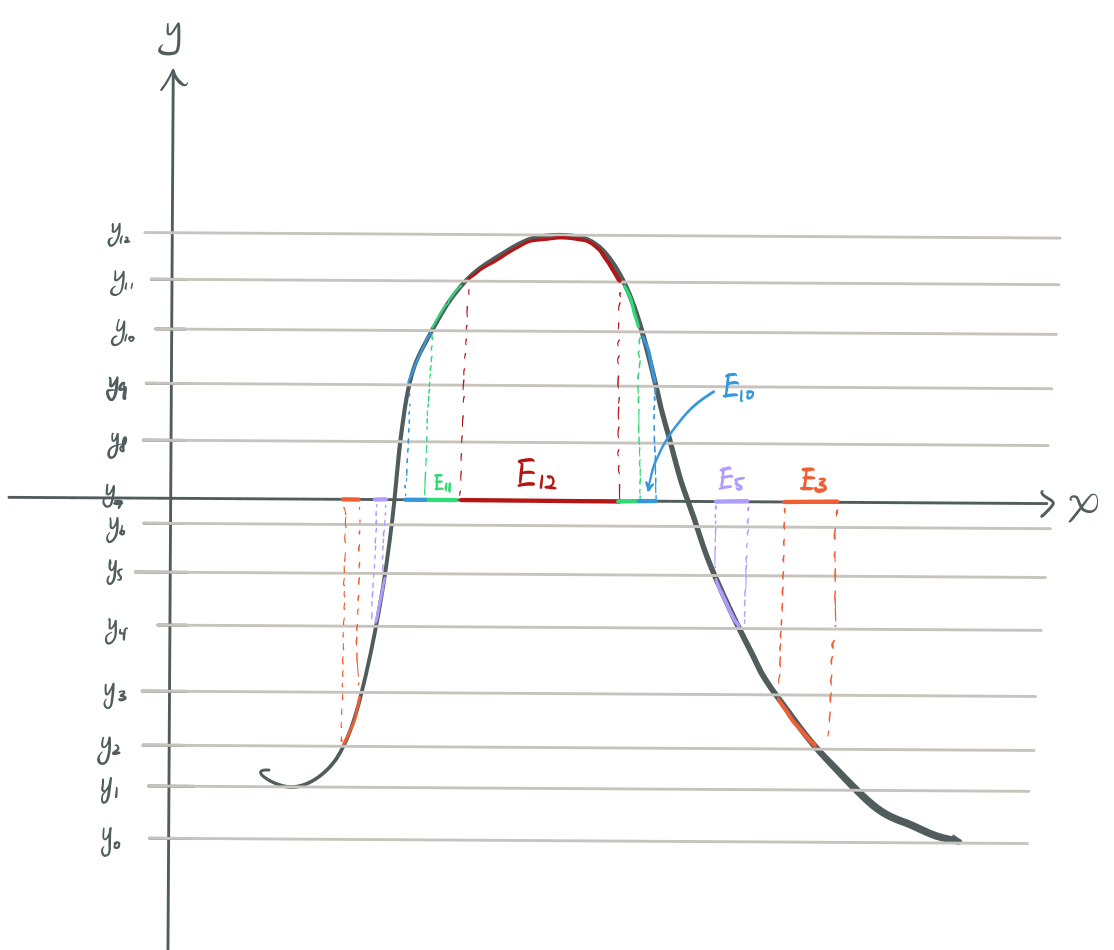
\includegraphics[width=0.5\linewidth]{images/heuristic_into_lesbesgue_integration.png}
  \caption{A sketch of what's happening with the construction of the $E_k$'s}
  \label{fig:a_sketch_of_what_s_happening_with_the_construction_of_the_e_k_s}
\end{figure*}

This will then allow us to estimate the integral of $f$ over $[a, b]$ by the
expression
\begin{equation*}
  \sum_{k=1}^{N} y_k m E_k,
\end{equation*}
where each of the $y_k m E_k$ are called \hlnotea{simple functions}. In the
expression, $mE_k$ denotes a ``measure'' \sidenote{Note that a measure is simply
a generalization of the notion of `length'.} of $E_k$.

\begin{figure*}[ht]
  \centering
  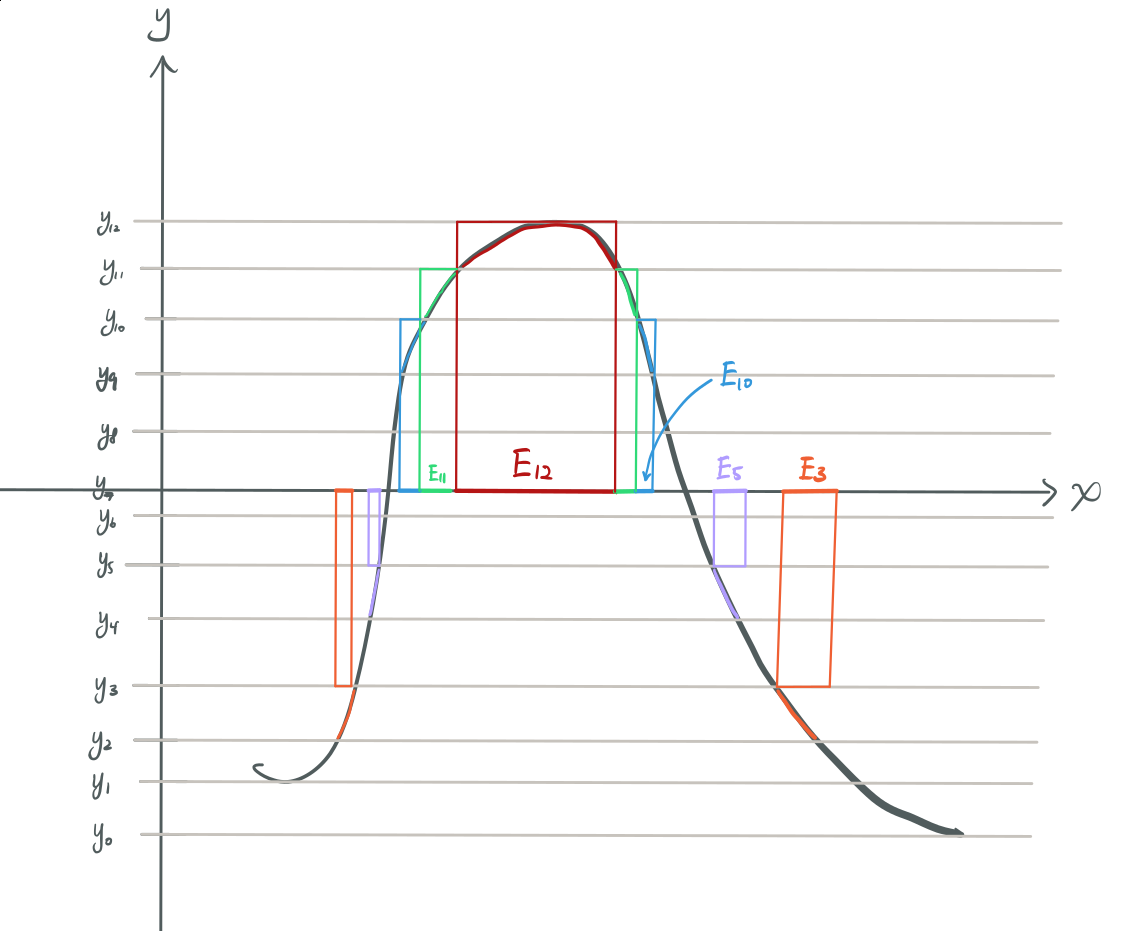
\includegraphics[width=0.5\linewidth]{images/heuristic_into_lesbesgue_integration_heaps.png}
  \caption{Drawing out the rectangles of $y_k mE_k$ from
  \cref{fig:a_sketch_of_what_s_happening_with_the_construction_of_the_e_k_s}.}
  \label{fig:drawing_out_the_rectangles_of_y_k_me_k_from_fig_}
\end{figure*}

We observe that $E_k$ need not be a particularly well-behaved set. However, note
that we may rearrange the possibly scattered pieces of each $E_k$ together, so
as to form a `continuous' base for the rectangle. We need our definition of a
measure to be able to capture this.

The following is an analogy from Lebesgue himself on comparing Lebesgue
integration and Riemann integration \cite{siegmund2008}:

\begin{quotebox}{magenta}{foreground}
  I have to pay a certain sum, which I have collected in my pocket. I take the
  bills and coins out of my pocket and give them to the creditor in the order I
  find them until I have reached the total sum. This is the Riemann integral.

  But I can proceed differently. After I have taken all the money out of my
  pocket I order the bills and coins according to identical values and then I
  pay the several heaps one after the other to the creditor. This is my
  integral.
\end{quotebox}

The insight here is that one can \hlbnotea{freely arrange} the values of te
functions, all the while \hlbnotea{preserving} the value of the integral.
\begin{itemize}
  \item This requires us to have a better understanding of what a measure is.
  \item This process of rearrangement converts certain functions which are
    extremely difficult to deal with, or outright impossible, with the Riemann
    integral, into easily digestible pieces using Lebesgue integral.
\end{itemize}

% section riemannian_integration_continued (end)

\section{Lebesgue Outer Measure}%
\label{sec:lebesgue_outer_measure}
% section lebesgue_outer_measure

\paragraph{Goals of the section}

\begin{enumerate}
  \item Define a ``measure of length'' on as many subsets of $\mathbb{R}$ as
    possible.
  \item The definition should agree with our intuition of what a `length' is.
\end{enumerate}

\begin{defn}[Length]\index{Length}\label{defn:length}
  For $a \leq b \in \mathbb{R}$, we define the \hlnoteb{length} of the interval
  $(a, b)$ to be $b - a$, and we write
  \begin{equation*}
    \ell((a, b)) \coloneqq b - a.
  \end{equation*}
  We also define
  \begin{itemize}
    \item $\ell(\emptyset) = 0$; and
    \item $\ell((a, \infty)) = \ell((-\infty, b)) = \ell((-\infty, \infty)) =
      \infty$.
  \end{itemize}
\end{defn}

\begin{defn}[Cover by Open Intervals]\index{Cover by Open Intervals}\label{defn:cover_by_open_intervals}
  Let $E \subseteq \mathbb{R}$. A countable collection $\{ I_n
  \}_{n=1}^{\infty}$ of open intervals is said to be a \hlnoteb{cover of $E$ by
  open intervals} if $E \subseteq \bigcup_{n=1}^{\infty} I_n$.
\end{defn}

\begin{note}
  In this course, the only covers that we shall use are \hlbnotec{open
  intervals}, and so we shall henceforth refer to the above simply as covers of
  $E$.
\end{note}

Before giving what immediately follows from the above, I shall present the
following notion of an outer measure.

\begin{defn}[Outer Measure]\index{Outer Measure}\label{defn:outer_measure}
  Let $\emptyset \neq X$ be a set. An \hlnoteb{outer measure} $\mu$ on $X$ is a
  function
  \begin{equation*}
    \mu : \mathcal{P}(X) \to [0, \infty] \coloneqq [0, \infty) \cup \{ \infty \}
  \end{equation*}
  which satisfies
  \begin{enumerate}
    \item $\mu \emptyset = 0$;
    \item (\hldefn{monotone increment} or \hldefn{monotonicity}) $E \subseteq F
      \subseteq X \implies \mu E \leq \mu F$; and
    \item (\hldefn{countable subadditivity} or
      \hldefn{$\sigma$-subadditivity}) $\{ E_n \}_{n=1}^{\infty} \subseteq
      \mathcal{P}(X)$
       \begin{equation*}
        \mu \left( \bigcup_{n=1}^{\infty} E_n \right) \leq \sum_{n=1}^{\infty}
        \mu E_n.
      \end{equation*}
  \end{enumerate}
\end{defn}

\begin{note}
  Note that by the monotonicity, the $\sigma$-subadditivity condition is
  equivalent to: given $\{ E_n \}_{n=1}^{\infty} \subseteq \mathcal{P}(X)$ and
  $F \subseteq \bigcup_{n=1}^{\infty} E_n$, we have that
  \begin{equation*}
    \mu(F) \leq \sum_{n=1}^{\infty} \mu(E_n).
  \end{equation*}
\end{note}

\begin{defn}[Lebesgue Outer Measure]\index{Lebesgue Outer Measure}\label{defn:lebesgue_outer_measure}
  We define the \hlnoteb{Lebesgue outer measure} as a function $m^* :
  \mathcal{P}(X) \to \mathbb{R}$ such that
  \begin{equation*}
    m^* E \coloneqq \inf \left\{ \sum_{n=1}^{\infty} \ell(I_n) : E \subseteq
    \bigcup_{n=1}^{\infty} I_n \right\}.
  \end{equation*}
\end{defn}

We cheated a little bit by calling the above an outer measure, so let us now
justify our cheating.

\begin{propo}[Validity of the Lebesgue Outer Measure]\label{propo:validity_of_the_lebesgue_outer_measure}
  $m^*$ is indeed an outer measure.
\end{propo}

\begin{proof}
  \hlbnoted{$\mu \emptyset = 0$} We consider a sequence of sets $\{ I_n
  \}_{n=1}^{\infty}$ such that $I_n = \emptyset$ for each $n = 1, \ldots,
  \infty$. It is clear that $\emptyset \subseteq \bigcup_{n=1}^{\infty} I_n$.
  Also, we have that $\ell(I_n) = 0$ for all $n = 1, \ldots, \infty$. It follows
  that
  \begin{equation*}
    0 \leq m^*(\emptyset) \leq \sum_{n=1}^{\infty} m^* (I_n) =
    \sum_{n=1}^{\infty} 0 = 0,
  \end{equation*}
  where the inequality is simply by the definition of $m^*$ being an infimum,
  \hlimpo{not to be confused with $\sigma$-subadditivity}. We thus have that
  \begin{equation*}
    m^*(\emptyset) = 0.
  \end{equation*}

  \noindent
  \hlbnoted{Monotonicity} Suppose $E \subseteq F \subseteq
  \mathbb{R}$, and $\{ I_n \}_{n=1}^{\infty}$ a cover of $F$. Then
  \begin{equation*}
    E \subseteq F \subseteq \bigcup_{n=1}^{\infty} I_n.
  \end{equation*}
  In particular, all covers of $F$ are also covers of $E$, i.e.
  \begin{equation*}
    \left\{ \{ J_m \}_{m=1}^{\infty} : E \subseteq \bigcup_{m=1}^{\infty} J_m \right\}
    \subseteq
    \left\{ \{ I_n \}_{n=1}^{\infty} : F \subseteq \bigcup_{n=1}^{\infty} I_n \right\}.
  \end{equation*}
  It follows that
  \begin{equation*}
    m^* E \leq m^* F.
  \end{equation*}

  \noindent
  \hlbnoted{$\sigma$-subaddivitity} Consider $\{ E_n \}_{n=1}^{\infty} \subseteq
  \mathcal{P}(X)$ such that $E \subseteq \bigcup_{n=1}^{\infty} E_n$. WTS
  \begin{equation*}
    m^* E \leq \sum_{n=1}^{\infty} m^* E_n.
  \end{equation*}

  Now if the sum of the RHS is infinite, i.e. if any of the $m^* E_n$ is
  infinite, then the inequality comes for free. Thus WMA $\sum_{n=1}^{\infty}
  E_n < \infty$, and in particular that $m^* E_n < \infty$ for all $n = 1,
  \ldots, \infty$.

  To do this, let $\epsilon > 0$. Since $m^* E_n < \infty$ for all $n$, we can
  find covers $\left\{ I_k^{(n)} \right\}_{k=1}^{\infty}$ for each of the
  $E_n$'s such that
  \begin{equation*}
    \sum_{k=1}^{\infty} \ell\left(I_k^{(n)}\right) < m^* E_n +
    \frac{\epsilon}{2^n}.
  \end{equation*}
  Then, we have that
  \begin{equation*}
    E \subseteq \bigcup_{n=1}^{\infty} E_n \subseteq \bigcup_{n=1}^{\infty}
    \bigcup_{k=1}^{\infty}  I_k^{(n)}.
  \end{equation*}
  Then by $m^* E$ being the infimum of the sum of lengths of the covering
  intervals, we have that
  \begin{align*}
    m^* E &\leq \sum_{n=1}^{\infty} \sum_{k=1}^{\infty} \ell \left( I_k^{(n)}
            \right) \\
          &\leq \sum_{n=1}^{\infty} \left( m^* E_n + \frac{\epsilon}{2^n}
            \right) \\
          &= \sum_{n=1}^{\infty} m^* E_n + \sum_{n=1}^{\infty}
            \frac{\epsilon}{2^n} \\
          &= \sum_{n=1}^{\infty} m^* E_n + \epsilon.
  \end{align*}
  Since $\epsilon$ was arbitrary, we have that
  \begin{equation*}
    m^* E_n \leq \sum_{n=1}^{\infty} m^* E_n,
  \end{equation*}
  as desired.
\end{proof}

\begin{crly}[Lebesgue Outer Measure of Countable Sets is Zero]\label{crly:lebesgue_outer_measure_of_countable_sets_is_zero}
  If $E \subseteq \mathbb{R}$ is countable, then $m^* E = 0$.
\end{crly}

\begin{proof}
  We shall prove for when $E$ is denumerable, for the finite case follows a
  similar proof. Let us write $E = \{ x_n \}_{n=1}^{\infty}$. Let $\epsilon > 0$ 
  and
  \begin{equation*}
    I_n = \left( x_n - \frac{\epsilon}{2^{n+1}},\, x_n + \frac{\epsilon}{2^{n+1}}
    \right).
  \end{equation*}
  Then it is clear that $\{ I_n \}_{n=1}^{\infty}$ is a cover of $E$.
  
  It follows that
  \begin{equation*}
    0 \leq m^* E \leq \sum_{n=1}^{\infty} \ell (I_n) = \sum_{n=1}^{\infty}
    \frac{\epsilon}{2^n} = \epsilon.
  \end{equation*}
  Thus as $\epsilon \to 0$, we have that
  \begin{equation*}
    m^* E = 0,
  \end{equation*}
  as expected.
\end{proof}

\begin{crly}[Lebesgue Outer Measure of $\mathbb{Q}$ is Zero]\label{crly:lebesgue_outer_measure_of_q_is_zero}
  We have that $m^* \mathbb{Q} = 0$.
\end{crly}

\newthought{In the proofs} above that we have looked into, and based on the
intuitive notion of the length of an open interval, it is compelling to simply
conclude that
\begin{equation*}
  m^* (a, b) = \ell(a, b) = b - a.
\end{equation*}
However, looking back at \cref{defn:lebesgue_outer_measure}, we know that that
is not how $m^* (a, b)$ is defined.

This leaves us with an interesting question:
\begin{quotebox}{green}{foreground}
  how does our notion of measure $m^*(a, b)$ of an interval compare with the
  notion of the length of an interval?
\end{quotebox}

By taking $I_1 = (a, b)$ and $I_n = \emptyset$ for $n \geq 2$, it is rather
clear that $\{ I_n \}_{n=1}^{\infty}$ is a cover of $(a, b)$, and so we have
\begin{equation}\label{eq:lebesgue_outer_measure_leq_length}
  m^* (a, b) \leq \ell(a, b) = b - a.
\end{equation}
However, the other side of the game is not as easy to confirm: we would have to
consider \hlimpo{all} possible covers of $(a, b)$, which is a lot.

Another question that we can ask ourselves seeing
\cref{eq:lebesgue_outer_measure_leq_length} is why can't $m^*(a, b)$ be
something that is strictly less than the length to give us an even more
`precise' measurement?

To answer these questions, it is useful to first consider the outer measure of a
closed and bounded interval, e.g. $[a, b]$, since these intervals are
\hlnotea{compact} under the \hlnotea{Heine-Borel Theorem}. This will give us a
finite subcover for every infinite cover of the compact interval, which is easy
to deal with.

We shall see that with the realization of the outer measure of a compact
interval, we will also be able to find the outer measure of intervals that are
neither open nor closed.

We shall prove the following proposition in the next lecture. Note that for the
sake of presentation, I shall abbreviate the Lebesgue Outer Measure as LOM.

\begin{propononum}[LOM of Arbitrary Intervals]
  Suppose $a < b \in \mathbb{R}$. Then
  \begin{enumerate}
    \item $m^*([a, b]) = b - a$; and therefore
    \item $m^*((a, b]) = m^*([a, b)) = m^*((a, b)) = b - a$.
  \end{enumerate}
\end{propononum}

% section lebesgue_outer_measure (end)

% chapter lecture_2_may_9th_2019 (end)

\chapter{Lecture 3 May 14th 2019}%
\label{chp:lecture_3_may_14th_2019}
% chapter lecture_3_may_14th_2019

\section{Lebesgue Outer Measure Continued}%
\label{sec:lebesgue_outer_measure_continued}
% section lebesgue_outer_measure_continued

\begin{propo}[LOM of Arbitrary Intervals]\label{propo:lom_of_arbitrary_intervals}
  Suppose $a < b \in \mathbb{R}$. Then
  \begin{enumerate}
    \item $m^*([a, b]) = b - a$; and therefore
    \item $m^*((a, b]) = m^*([a, b)) = m^*((a, b)) = b - a$.
  \end{enumerate}
\end{propo}

\begin{proof}
  \begin{enumerate}
    \item Consider $a < b \in \mathbb{R}$. Let $\epsilon > 0$, and let
      \begin{equation*}
        I_1 = \left( a - \frac{\epsilon}{2}, \, b + \frac{\epsilon}{2} \right)
      \end{equation*}
      and $I_n = \emptyset$ for $n \geq 2$. Then $\{ I_n \}_{n=1}^{\infty}$ is a
      cover of $[a, b]$. This means that
      \begin{equation*}
        m^*([a, b]) \leq \sum_{n=1}^{\infty} \ell(I_n) = b - a + \epsilon.
      \end{equation*}
      So for all $\epsilon \to 0$, we have that
      \begin{equation*}
        m^*([a, b]) \leq b - a.
      \end{equation*}

      \sidenote{For the converse, we know that $m^*([a, b]) = \inf \faStar$,
      where $\faStar$ is just a placeholder for you-know-what. So $m^*([a,
      b])$ is one of the sums. So if we can show that for an arbitrary sum,
      $\geq$ holds, our work is done.} Conversely, if $[a, b]$ is covered by open
      intervals $\{ I_n \}_{n=1}^{\infty}$, then by compactness of $[a, b]$ (via
      the \hlnotea{Heine-Borel Theorem}), we know that we can cover $[a, b]$ by
      finitely many of these intervals, and let us denote these as $\{ I_n
      \}_{n=1}^{N}$, for some $1 \leq N < \infty$.

      WTS
      \begin{equation*}
        \sum_{n=1}^{N} \ell(I_n) \geq b - a.
      \end{equation*}
      If LHS $= \infty$, then our work is done. Thus wlog, WMA each $I_n = (a_n,
      b_n)$ is a finite interval. Note that we have
      \begin{equation*}
        [a, b] \subseteq \bigcup_{n=1}^{N} (a_n, b_n).
      \end{equation*}
      In particular, $a \in \bigcup_{n=1}^{N} I_n$. Thus, $\exists 1 \leq n_2
      \leq N$ such that $a \in I_{n_1}$. Now if $b_{n_1} > b$, we shall stop
      this process for our work is done, since then $[a, b] \subseteq I_{n_1}$.
      Otherwise, if $b_{n_1} \leq b$, then $b_{n_1} \in [a, b] \subseteq
      \bigcup_{n=1}^{N} I_n$, which means that $\exists 1 \leq n_2 \leq N$ such
      that $b_{n_1} \in I_{n_2}$.
      \begin{figure*}[ht]
        \centering
        \begin{tikzpicture}
          \draw (-7, 0) -- (7, 0);
          \draw (-4, 0.2) -- (-4, -0.2) node[below] {$a$};
          \draw (4, 0.2) -- (4, -0.2) node[below] {$b$};
          \draw[
            {Arc Barb[length=5pt,width=15pt]}-{Arc Barb[length=5pt,width=15pt]},red
            ] (-5,0) node[above=10pt] {$a_{n_1}$} -- (-2,0) node[above=10pt]
            {$b_{n_1}$};
          \draw[
            {Arc Barb[length=5pt,width=15pt]}-{Arc Barb[length=5pt,width=15pt]},cyan
            ] (-3,0) node[above=10pt] {$a_{n_2}$} -- (0,0) node[above=10pt]
            {$b_{n_2}$};
          \node at (1, 0.6) {$\hdots$};
          \draw[
            {Arc Barb[length=5pt,width=15pt]}-{Arc Barb[length=5pt,width=15pt]},magenta
            ] (2,0) node[above=10pt] {$a_{n_k}$} -- (5,0) node[above=10pt]
            {$b_{n_k}$};
        \end{tikzpicture}
        \caption{Our continual picking of $I_{n_1}, I_{n_2}, \ldots, I_{n_k}$}
        \label{fig:our_continual_picking_of_i__n_1_i__n_2_ldots_i__n_k_}
      \end{figure*}
      Notice that $n_1 \neq n_2$, since $b_{n_1} \notin I_{n_1}$ but $b_{n_1}
      \in I_{n_2}$.

      Now once again, if $b_{n_2} > b$, then we shall stop this process since
      our work is done. Otherwise, we have $a < b_{n_2} \leq b$, and so $\exists
      1 \leq n_3 \leq N$, $n_3 \neq n_1, n_2$, such that $b_{n_2} \in I_3$...

      We continue with the above process for as long as $b_{n_k} \leq b$. We can
      thus find, for each $k$, $I_{n_{k+1}}$, where $n_{k+1} \in \{ 1, \ldots, N
      \} \setminus \{ n_1, n_2, \ldots, n_k \}$, such that $b_{n_k} \in
      I_{n_{k+1}}$.

      However, since each of the $I_{n_k}$'s are different, and since we only
      have $N$ such intervals, there must exists a $K \leq N$ such that
      \begin{equation*}
        b_{n_{K-1}} \leq b \text{ and } b_{n_K} > b.
      \end{equation*}

      It now suffices for us to show that
      \begin{equation*}
        \sum_{j=1}^{K} \ell(I_{n_j}) \geq b - a.
      \end{equation*}

      Observe that
      \begin{align*}
        \sum_{j=1}^{K} \ell(I_{n_j})
        &= (b_{n_K} - a_{n_K}) + (b_{n_{K-1}} - a_{n_{K-1}}) + \hdots \\
        &\quad + (b_{n_2} - a_{n_2}) + (b_{n_1} - a_{n_1}) \\
        &= b_{n_K} + \underset{\geq 0}{(b_{n_{K-1}} - a_{n_K})} + \underset{\geq
          0}{(b_{n_{K-2}} - a_{n_{K-1}})} + \hdots \\
        &\quad + \underset{\geq 0}{(b_{n_1} - a_{n_2})} - a_{n_1} \\
        &\geq b_{n_K} - a_{n_1} \geq b - a.
      \end{align*}
      Thus
      \begin{equation*}
        \sum_{n=1}^{\infty} \ell(I_n) \geq \sum_{n=1}^{N} \ell(I_n) \geq
        \sum_{j=1}^{K} \ell(I_{n_j}) \geq b - a,
      \end{equation*}
      whence
      \begin{equation*}
        m^*([a, b]) \geq b - a.
      \end{equation*}

      It follows that, indeed,
      \begin{equation*}
        m^*([a, b]) = b - a.
      \end{equation*}

    \item First, note that
      \begin{equation*}
        m^*((a, b)) \leq m^*([a, b]) \leq b - a.
      \end{equation*}
      On the other hand, notice that $\forall 0 < \epsilon < \frac{b - a}{2}$,
      we have that
      \begin{equation*}
        [a + \epsilon, b - \epsilon] \subseteq (a, b),
      \end{equation*}
      and so by monotonicity,
      \begin{equation*}
        (b - a) - 2 \epsilon = m^*([a + \epsilon, b - \epsilon]) \leq m^*((a,
        b)).
      \end{equation*}
      As $\epsilon \to 0$, we have that
      \begin{equation*}
        b - a \leq m^*((a, b)) \leq b - a.
      \end{equation*}
      So
      \begin{equation*}
        m^*((a, b)) = b - a
      \end{equation*}
      as desired.

      Finally, we have that
      \begin{equation*}
        b - a = m^*((a, b)) \leq m^*((a, b]) \leq m^*([a, b]) = b - a,
      \end{equation*}
      and similarly
      \begin{equation*}
        b - a = m^*((a, b)) \leq m^*([a, b)) \leq m^*([a, b]) = b - a.
      \end{equation*}
      Thus
      \begin{equation*}
        m^*((a, b)) = m^*((a, b]) = m^*([a, b)) = b - a
      \end{equation*}
      as required.
  \end{enumerate}
\end{proof}

\begin{propo}[LOM of Infinite Intervals]\label{propo:lom_of_infinite_intervals}
  We have that $\forall a, b \in \mathbb{R}$,
  \begin{align*}
    m^*((a, \infty)) &= m^*([a, \infty)) \\
                     &= m^*((-\infty, b)) = m^*((-\infty, b]) \\
                     &= m^* \mathbb{R} = \infty.
  \end{align*}
\end{propo}

\begin{proof}
  Observe that
  \begin{equation*}
    (a, a + n) \subseteq (a, \infty)
  \end{equation*}
  for all $n \geq 1$. Thus
  \begin{equation*}
    n = m^*((a, a + n)) \leq m^*((a, \infty))
  \end{equation*}
  for all $n \geq 1$. Hence
  \begin{equation*}
    m^*((a, \infty)) = \infty
  \end{equation*}
  by definition.

  All other cases follow similarly.
\end{proof}

\begin{crly}[Uncountability of $\mathbb{R}$]\label{crly:uncountability_of_r}
  $\mathbb{R}$ is uncountable.
\end{crly}

\begin{proof}
  We have that
  \begin{equation*}
    m^* \mathbb{R} = \infty \neq 0,
  \end{equation*}
  and so it follows from
  \cref{crly:lebesgue_outer_measure_of_countable_sets_is_zero}, we must have
  that $\mathbb{R}$ is uncountable.
\end{proof}

\begin{defn}[Translation Invariant]\index{Translation Invariant}\label{defn:translation_invariant}
  Let $\mu$ be an \hyperref[defn:outer_measure]{outer measure} on $\mathbb{R}$.
  We say that $\mu$ is \hlnoteb{translation invariant} if $\forall E \subseteq
  \mathbb{R}$,
  \begin{equation*}
    \mu(E) = \mu(E + \kappa)
  \end{equation*}
  for all $\kappa \in \mathbb{R}$, where
  \begin{equation*}
    E + \kappa \coloneqq \{ x + \kappa : x \in E \}.
  \end{equation*}
\end{defn}

\begin{propo}[Translation Invariance of the LOM]\label{propo:translation_invariance_of_the_lom}
  The Lebesgue outer measure is translation invariant.
\end{propo}

\begin{proof}
  Let $E \subseteq \mathbb{R}$ and $\kappa \in \mathbb{R}$. Note that $E$ is
  covered by open intervals $\{ I_n \}_{n=1}^{\infty}$ iff $E + \kappa$ is
  covered by $\{ I_n + \kappa \}_{n=1}^{\infty}$.

  \noindent
  \hlbnoted{Claim: $\forall n \geq 1$, $\ell(I_n + \kappa) = \ell(I_n)$} Write
  \begin{equation*}
    I_n = (a_n, b_n).
  \end{equation*}
  Then
  \begin{equation*}
    I_n + \kappa = (a_n + \kappa, b_n + \kappa).
  \end{equation*}
  Observe that
  \begin{equation*}
    \ell(I_n + \kappa) = b_n + \kappa - (a_n - \kappa) = b_n - a_n = \ell(I_n),
  \end{equation*}
  as claimed. $\dashv$

  By the claim, it follows that
  \begin{align*}
    m^*(E) &= \inf \left\{ \sum_{n=1}^{\infty} \ell(I_n) : E \subseteq
            \bigcup_{n=1}^{\infty} \right\} \\
           &= \inf \left\{ \sum_{n=1}^{\infty} \ell(I_n + \kappa) : E + \kappa \subseteq
           \bigcup_{n=1}^{\infty} (I_n + \kappa)  \right\} \\
           &= m^*(E + \kappa).
  \end{align*}
\end{proof}

\begin{remark}
  Suppose $E \subseteq \mathbb{R}$ and $E = \bigcup_{n=1}^{\infty} E_n$,
  where
  \begin{equation*}
    E_i \cap E_j = \emptyset \text{ if } i \neq j.
  \end{equation*}
  Now by $\sigma$-subadditivity of $m^*$, we have that
  \begin{equation*}
    m^* E \leq \sum_{n=1}^{\infty} m^* E_n.
  \end{equation*}

  However, equality is not guaranteed. Consider the following case: if $E = [0,
  1]$, we may have $E_n = [0, 1]$ for all $n >= 1$, in which case $E =
  \bigcup_{n=1}^{\infty} E_n = [0, 1]$, but
  \begin{equation*}
    m^* E = m^* [0, 1] = 1 < \infty = \sum_{n=1}^{\infty} m^* E_n.
  \end{equation*}

  It would be desirable to have
  \begin{equation*}
    m^* E = \sum_{n=1}^{\infty} m^* E_n,
  \end{equation*}
  when the $E_i$'s are pairwise disjoint, i.e. $E = \bigcupdot_{n=1}^{\infty}
  E_n$. In fact, this would agree with our intuition, that if the outer measure
  is going to be our `length'. Consider the example $A = [0, 2] \cup [5, 7]$.
  Then we would expect $m^* A = 2 + 2 = 4$.

  However, this is actually impossible for an arbitrary number of collections.
\end{remark}

\begin{thm}[Non-existence of a sensible Translation Invariant Outer Measure that is also $\sigma$-additive]\label{thm:non_existence_of_a_sensible_translation_invariant_outer_measure_that_is_also_sigma_additive}
  There does not exist a translation-invariant outer measure $\mu$ on
  $\mathbb{R}$ that satisfies
  \begin{enumerate}
    \item $\mu(\mathbb{R}) > 0$;
    \item $\mu[0, 1] < \infty$; and
    \item $\mu$ is \hldefn{$\sigma$-additive}; i.e. if $\{ E_n
      \}_{n=1}^{\infty}$ is a countable collection of disjoint subsets of
      $\mathbb{R}$ that covers $E \subseteq \mathbb{R}$, then
      \begin{equation*}
        \mu E = \sum_{n=1}^{\infty} \mu E_n.
      \end{equation*}
  \end{enumerate}
  Consequently, the \hyperref[defn:lebesgue_outer_measure]{Lebesgue outer
  measure} $m^*$ is \hlimpo{not} $\sigma$-additive.
\end{thm}

\begin{proof}
  Suppose to the contrary that such a $\mu$ exists.

  \noindent
  \hlbnoteb{Step 1} Consider the relation $\sim$ on $\mathbb{R}$ such that $x
  \sim y$ if $x - y \in \mathbb{Q}$.

  \noindent
  \hlbnoted{Claim: $\sim$ is an equivalence relation}
  \begin{itemize}
    \item (\textbf{reflexivity}) We know that $0 \in \mathbb{Q}$ and $x - x = 0$.
      Thus $x \sim x$.
    \item (\textbf{symmetry}) Since $\mathbb{Q}$ is a \hlnotea{field}, it is
      closed under multiplication, and $-1 \in \mathbb{Q}$. Thus if $x \sim y$,
      then $x - y \in \mathbb{Q}$, and so $(-1)(x - y) = y - x \in \mathbb{Q}$,
      which means $y \sim x$.
    \item (\textbf{transitivity}) Again, since $\mathbb{Q}$ is a field, it is
      closed under (this time) addition. Thus
      \begin{align*}
        &x \sim y \, \land \, y \sim z \implies (x - y), \, (y - z) \in
        \mathbb{Q} \\
        &\implies (x - y) + (y - z) = x - z \in \mathbb{Q}.
      \end{align*}
      Thus $x \sim z$.
  \end{itemize}
  This proves the claim. $\dashv$

  Let
  \begin{equation*}
    [x] \coloneqq x + \mathbb{Q} \coloneqq \{ x + q : q \in \mathbb{Q} \}
  \end{equation*}
  denote the equivalence class of $x$ wrt $\sim$. Note that the set of
  equivalence classes, which we shall represent as
  \begin{equation*}
    \mathcal{F} \coloneqq \{ [x] : x \in \mathbb{R} \},
  \end{equation*}
  partitions $\mathbb{R}$, i.e.
  \begin{itemize}
    \item $[x] = [y] \iff x - y \in \mathbb{Q}$; and
    \item $[x] \cap [y] = \emptyset$ otherwise.
  \end{itemize}

  Note that since $\mathbb{Q}$ is \hlnotea{dense} in $\mathbb{R}$, we have that
  $[x] = x + \mathbb{Q}$ is also dense in $\mathbb{R}$, for all $x \in
  \mathbb{R}$. Then for each \sidenote{Notice that here, we
  have invoked the \hlbnotee{Axiom of Choice}.} $F \in \mathcal{F}$, $\exists
  x_F \in F$ such that
  \begin{equation*}
    0 \leq x_F \leq 1.
  \end{equation*}
  Now consider the set
  \begin{equation*}
    \mathbb{V} \coloneqq \{ x_F : F \in \mathcal{F} \} \subseteq [0, 1],
  \end{equation*}
  which is called \hldefn{Vitali's Set}.

  \noindent
  \hlbnoteb{Step 2} Since $\mathcal{F}$ partitions $\mathbb{R}$, we have that
  \begin{align*}
    \mathbb{R} &= \bigcupdot_{F \in \mathcal{F}} F = \bigcupdot_{F \in
                 \mathcal{F}} [x_F] \\
               &= \bigcupdot_{F \in \mathcal{F}} x_F + \mathbb{Q} \\
               &= \mathbb{V} + \mathbb{Q} \coloneqq \{ x + q : q \in \mathbb{Q},
                x \in \mathbb{V} \}.
  \end{align*}

  \noindent
  \hlbnoteb{Step 3} \hlbnoted{Claim: $p \neq q \in \mathbb{Q} \implies
  (\mathbb{V} + p) \cap (\mathbb{V} + q) = \emptyset$} Suppose not, and suppose
  $\exists y \in (\mathbb{V} + p) \cap (\mathbb{V} + q)$. Then $\exists F_1, F_2
  \in \mathcal{F}$ such that
  \begin{equation}\label{eq:nonexistence_of_transinvar_outmea_eq1}
    y = x_{F_1} + p = x_{F_2} + q.
  \end{equation}
  Then we may rearrange the above equation to get
  \begin{equation*}
    x_{F_1} - x_{F_2} = q - p \in \mathbb{Q}.
  \end{equation*}
  This implies that
  \begin{equation*}
    [x_{F_1}] = [x_{F_2}] \implies F_1 = F_2
  \end{equation*}
  since $\mathbb{V}$ consists of one unique representative from each of the
  equivalence classes. However, this would mean that
  \begin{equation*}
    x_{F_1} = x_{F_2}.
  \end{equation*}
  Since $p \neq q$, we have that
  \begin{equation*}
    x_{F_1} + p \neq x_{F_2} + q,
  \end{equation*}
  which contradicts \cref{eq:nonexistence_of_transinvar_outmea_eq1}. Thus
  \begin{equation*}
    (\mathbb{V} + p) \cap (\mathbb{V} + q) = \emptyset,
  \end{equation*}
  as claimed. $\dashv$

  This in turn means that the $\mathbb{V} + q$, for each $q \in \mathbb{Q}$,
  also partitions $\mathbb{R}$. In other words, if we write $\mathbb{Q} = \{ p_n
  \}_{n=1}^{\infty}$, then
  \begin{equation*}
    \mathbb{R} = \mathbb{V} + \mathbb{Q} = \bigcupdot_{n=1}^{\infty} \mathbb{V}
    + p_n.
  \end{equation*}

  Now, note that
  \begin{equation*}
    0 \neq \mu \mathbb{R} \overset{(1)}{=} \sum_{n=1}^{\infty} \mu(\mathbb{V} +
    p_n) \overset{(2)}{=} \sum_{n=1}^{\infty} \mu(\mathbb{V}),
  \end{equation*}
  where $(1)$ is by $\mu$ being $\sigma$-additive and $(2)$ is by $\mu$ being
  translation invariant, both directly from our assumptions. This means that
  \begin{equation*}
    \mu \mathbb{V} > 0.
  \end{equation*}

  \noindent
  \hlbnoteb{Step 4} Now consider $S = \mathbb{Q} \cap [0, 1]$ such that $S$ is
  denumerable. Write
  \begin{equation*}
    S = \{ s_n \}_{n=1}^{\infty}.
  \end{equation*}
  Note that for all $n \geq 1$,
  \begin{equation*}
    \mathbb{V} \subseteq [0, 1] \implies \mathbb{V} + s_n \subseteq [0, 2],
  \end{equation*}
  and as proven above
  \begin{equation*}
    i \neq j \implies (\mathbb{V} + s_i) \cap (\mathbb{V} + s_j) = \emptyset.
  \end{equation*}

  Thus it follows that
  \begin{equation*}
    \mu \left( \bigcupdot_{n=1}^{\infty} \mathbb{V} + s_n \right)
    = \sum_{n=1}^{\infty} \mu (\mathbb{V} + s_n) 
    = \sum_{n=1}^{\infty} \mu(\mathbb{V})
    = \infty.
  \end{equation*}
  Also,
  \begin{align*}
    \mu \left( \bigcupdot_{n=1}^{\infty} \mathbb{V} + s_n \right)
    &= \sum_{n=1}^{\infty} \mu (\mathbb{V} + s_n) \\
    &\leq \mu([0, 2]) = \mu([0, 1] \cup ([0, 1] + 1)) \\
    &\leq \mu[0, 1] + \mu([0, 1] + 1) \\
    &= 2 \mu([0, 1]) = 2 < \infty,
  \end{align*}
  contradicting what we have right above.

  Therefore, no such $\mu$ exists.
\end{proof}

With the realization of
\cref{thm:non_existence_of_a_sensible_translation_invariant_outer_measure_that_is_also_sigma_additive},
we find ourselves facing a losing dilemma: we may either
\begin{enumerate}
  \item be happy with the Lebesgue outer measure $m^*$ for \hlbnotee{all}
    subsets $E \subseteq \mathbb{R}$, which would \hlbnotec{agree with our
    intuitive notion} of length, at the price of $\sigma$-additivity; or
  \item restrict the \hlbnotee{domain} of our function $m^*$ to some family of
    subsets of $\mathbb{R}$, where $m^*$ would have $\sigma$-additivity.
\end{enumerate}

We shall adopt the second approach. We shall call the collection of sets where
$m^*$ has $\sigma$-additivity as the collection of \hlnotea{Lebesgue measurable
sets}.

% section lebesgue_outer_measure_continued (end)

\section{Lebesgue Measure}%
\label{sec:lebesgue_measure}
% section lebesgue_measure

We shall first introduce \hlnotea{Carath\'{e}odory's} definition of a Lebesgue
measurable set.

\begin{defn}[Lebesgue Measureable Set]\index{Lebesgue Measureable Set}\label{defn:lebesgue_measureable_set}
  A set $E \subseteq \mathbb{R}$ is said to be \hlnoteb{Lebesgue measurable} if,
  $\forall X \subseteq \mathbb{R}$,
  \begin{equation*}
    m^* X = m^* ( X \cap E ) + m^* (X \setminus E).
  \end{equation*}
  We denote the collection of all Lebesgue measurable sets as
  $\mathfrak{M}(\mathbb{R})$.
\end{defn}

\begin{remark}
  Since we shall almost exclusively focus on the Lebesgue measure, we shall
  hereafter refer to ``Lebesgue measurable sets'' as simply ``measurable sets''.
\end{remark}

\begin{note}
  I shall quote and paraphrase this remark from our course notes
  \cite{marcoux2018}:
  \begin{quotebox}{magenta}{foreground}
    Informally, we see that a set $E \subseteq \mathbb{R}$ is measurable
    provided that it is a ``universal slicer'', that it ``slices'' every other
    set $X$ into two \hlwarn{disjoint} sets, into where the Lebesgue outer
    measure is \hlimpo{$\sigma$-additive}.
  \end{quotebox}

  Also, note that we get the following inequality for free, simply from
  $\sigma$-subadditivity of $m^*$:
  \begin{equation*}
    m^* X \leq m^* (X \cap E) + m^* (X \setminus E).
  \end{equation*}
  Thus, it suffices for us to check if the reverse inequality holds for all sets
  $X \subseteq \mathbb{R}$.
\end{note}

Before ploughing forward to getting out hands dirty with examples, let us first
study a result on a structure of $\mathfrak{M}(\mathbb{R})$ that is rather
interesting. \sidenote{For those who has dirtied themselves in the world of
probability and statistics, especially probability theory, get ready to get
excited!}

\begin{defn}[Algebra of Sets]\index{Algebra of Sets}\index{$\sigma$-algebra of Sets}\label{defn:algebra_of_sets}\label{defn:sigma_algebra_of_sets}
  A collection $\Omega \subseteq \mathcal{P}(\mathbb{R})$ is said to be an
  \hlnoteb{algebra of sets} if
  \begin{enumerate}
    \item $\mathbb{R} \in \Omega$;
    \item (\textbf{closed under complementation}) $E \in \Omega \implies E^C \in
      \Omega$; and
    \item (\textbf{closed under finite union}) given $N \geq 1$ and $\{ E_n
      \}_{n=1}^{N} \subseteq \Omega$, then
      \begin{equation*}
        \bigcup_{n=1}^{N} E_n \in \Omega.
      \end{equation*}
  \end{enumerate}
  We say that $\Omega$ is a \hlnoteb{$\sigma$-algebra of sets} if
  \begin{enumerate}
    \item $\Omega$ is an algebra of sets; and
    \item (\textbf{closed under countable union}) if $\{ E_n \}_{n=1}^{\infty}
      \subseteq \Omega$, then
      \begin{equation*}
        \bigcup_{n=1}^{\infty} E_n \in \Omega.
      \end{equation*}
  \end{enumerate}
\end{defn}

\begin{note}
  We often call a $\sigma$-algebra of sets as simply a $\sigma$-algebra.
\end{note}

\begin{thm}[$\mathfrak{M}(\mathbb{R})$ is a $\sigma$-algebra]\label{thm:_m_r_is_a_sigma_algebra} 
  The collection $\mathfrak{M}(\mathbb{R})$ of Lebesgue measurable sets in
  $\mathbb{R}$ is a $\sigma$-algebra.
\end{thm}

\begin{proof}
  \hlwarn{Proof to be completed after the next lecture.}
\end{proof}

% section lebesgue_measure (end)

% chapter lecture_3_may_14th_2019 (end)

\appendix

\backmatter

\fancyhead[LE]{\thepage \enspace \textsl{\leftmark}}

\bibliography{references}

\printindex

\end{document}
% vim:tw=80:fdm=syntax
